\chapter{Introduction to data}
\label{introductionToData}

%\begin{tipBox}{\tipBoxTitle[Chapter Goal:]{Thinking about data}
%Understand basics about data organization, data types, numerical summaries of data, graphical summaries of data, and foundational techniques for data collection. We begin and end the chapter with case studies.}
%\end{tipBox}

Scientists seek to answer questions using rigorous methods and careful observations. These observations -- collected from the likes of field notes, surveys, and experiments -- form the backbone of a statistical investigation and are called \term{data}. Statistics is the study of how best to collect, analyze, and draw conclusions from data. It is helpful to put statistics in the context of a general process of investigation:
\begin{enumerate}
\setlength{\itemsep}{0mm}
\item Identify a question or problem.
\item Collect relevant data on the topic.
\item Analyze the data.
\item Form a conclusion.
%\item Make decisions based on the conclusion.
\end{enumerate}
Statistics as a subject focuses on making stages (2)-(4) objective, rigorous, and efficient. That is, statistics has three primary components: How best can we collect data? How should it be analyzed? And what can we infer from the analysis?

The topics scientists investigate are as diverse as the questions they ask. However, many of these investigations can be addressed with a small number of data collection techniques, analytic tools, and fundamental concepts in statistical inference. This chapter provides a glimpse into these and other themes we will encounter throughout the rest of the book. We introduce the basic principles of each branch and learn some tools along the way. We will encounter applications from other fields, some of which are not typically associated with science but nonetheless can benefit from statistical study.

\section[Case study]{Case study: using stents to prevent strokes}
\label{basicExampleOfStentsAndStrokes}

\index{data!stroke|(}

%We first consider a scientific study to introduce basic ideas about data collection, summary, and conclusions. While we encourage the reader to think about each of the bolded terms, we will revisit all terms in greater detail later this chapter.

Section~\ref{basicExampleOfStentsAndStrokes} introduces a classic challenge in statistics: evaluating the efficacy of a pharmaceutical treatment. Terms in this section, and indeed much of this chapter, will all be revisited later in the text, and in greater detail. The plan for now is simply to begin getting a sense of the role statistics can play in practice.

In this first section, we consider an experiment to study the effectiveness of stents in treating patients at risk of stroke\footnote{Chimowitz MI, Lynn MJ, Derdeyn CP, et al. 2011. Stenting versus Aggressive Medical Therapy for Intracranial Arterial Stenosis. New England Journal of Medicine 365:993-1003. \url{http://www.nejm.org/doi/full/10.1056/NEJMoa1105335}. NY Times article reporting on the study: \url{http://www.nytimes.com/2011/09/08/health/research/08stent.html}.}.
%Anturane Reinfarction Trial Research Group. 1980. Sulfinpyrazone in the prevention of sudden death after myocardial infarction. New England Journal of Medicine 302(5):250-256.}.
Stents are devices to put inside blood vessels that assist in patient recovery after cardiac events and reduce the risk of additional an heart attack or death. Many doctors have hoped that there would be similar benefits for patients at risk of stroke. We start by writing the principle question the researchers hope to answer:
\begin{quote}
Does the use of stents reduce the risk of stroke?
\end{quote}

The researchers who asked this question collected data on 451 at-risk patients. Each volunteer patient was randomly assigned to one of two groups:
\begin{itemize}
\item[]\termsub{Treatment group}{treatment group}. Patients in the treatment group received a stent and aggressive medical management. The aggressive medical management included medications, management of risk factors, and help in lifestyle modification.
\item[]\termsub{Control group}{control group}. Patients in the control group received aggressive medical management only. This medical management was identical in each group.
\end{itemize}
There were 224 patiens assigned to the treatment group and 227 to the control group. The \term{control group} is used to set a baseline or reference to compare with the \term{treatment group}.

Patients were specifically classified at two time points: 30~days after enrollment and 365~days after enrollment. If a patient had a stroke by the end of a time period, they were given the label \resp{stroke}, otherwise they were given the label \resp{no\_event}. The results of 5 patients are summarized in Table~\ref{stentStudyResultsDF}.
\begin{table}[h]
\centering
\begin{tabular}{l ccc}
\hline
Patient	&	group	&	0-30 days 	&	0-365 days \\
\hline
1		&	\resp{treatment} &	\resp{no\_event} &	\resp{no\_event} \\
2		&	\resp{treatment} &	\resp{stroke} & \resp{stroke} \\
3		&	\resp{treatment} &	\resp{no\_event} & \resp{no\_event} \\
$\vdots$	&	$\vdots$	  &	$\vdots$ \\
450	&	\resp{control} &	\resp{no\_event} &	\resp{no\_event} \\
451	&	\resp{control} &	\resp{no\_event} &	\resp{no\_event} \\
\hline
\end{tabular}
\caption{Results for five patients from the stent study.}
\label{stentStudyResultsDF}
% trmt <- c(rep('trmt', 224), rep('control', 227)); outcome30 <- c(rep(c('event', 'no_event'), c(33, 191)), rep(c('event', 'no_event'), c(13, 214))); outcome365 <- c(rep(c('event', 'no_event'), c(33, 191)), rep(c('event', 'no_event'), c(13, 214)))
\end{table}

Considering data from each patient individually would be a long, cumbersome path towards answering the original research question. Instead, it is often more useful to perform a data analysis, considering all of the data at once. We first might summarize the raw data in a more helpful way, like that shown in Table~\ref{stentStudyResults}. In this table, we can quickly see what happened over the entire study. For instance, to identify the number of patients in the treatment group who had a stroke by 30 days, we look in the left-side of the table at the intersection of the \resp{treatment} and \resp{stroke}: 33.
\begin{table}[h]
\centering
\begin{tabular}{l l cc c cc c}
& \multicolumn{2}{c}{0-30 days} &\hspace{5mm}\ & \multicolumn{2}{c}{0-365 days} \\ %& \hspace{3mm}\ &  \\
  \cline{2-3} \cline{5-6}
	& 	\resp{stroke} 	& \resp{noEvent} && 	\resp{stroke} 	& \resp{noEvent} \\ %&& Total  \\ 
  \hline
\resp{treatment} 	& 33		& 191	&&	45 	& 179	\\ %&&	224 \\
\resp{control} 		& 13		& 214	&& 	28	& 199	\\ %&&	227 \\ 
  \hline
Total				& 46		& 405	&&	73	& 378	\\ %&&	451 \\
  \hline
\end{tabular}
\caption{Descriptive statistics for the stent study.}
\label{stentStudyResults}
\end{table}

\begin{exercise}
Of the 224 patients in the treatment group, 45 had a stroke by the end of the first year. Using these two numbers, compute the proportion of patients in the treatment group who had a stroke by the end of their first year. Answer in the footnote\footnote{The proportion of the 224 patients who had a stroke within 365 days: $45/224 = 0.20$.}.
\end{exercise}

We can compute summary statistics from the summary table. A \term{summary statistic} is a single number summarizing a large amount of data\footnote{Formally, a summary statistic is a value computed from the data. Some summary statistics are more useful than others.}. For instance, the primary results of the study after 1~year could be placed in two summary statistics: the proportion of people who had a stroke in each group. %You've already computed one of these values.
\begin{itemize}
\setlength{\itemsep}{0mm}
\item[] Proportion who had a stroke in the treatment (stent) group: $45/224 = 0.20 = 20\%$.
\item[] Proportion who had a stroke in the control group: $28/227 = 0.12 = 12\%$.
\end{itemize}
These two summary statistics are useful in looking for differences in the groups, and we are in for a surprise: an additional 8\% of patients in the treatment group had a stroke! This is important for two reasons. First, it is contrary to what doctors expected, which was that stents would \emph{reduce} the rate of strokes. Second, it leads to a statistical question: do the data show a ``real'' difference between the groups?

This question is subtle. Suppose you flip a coin 100 times. While the chance it is heads in any given coin flip is 50\%, we probably won't observe exactly 50 heads but we will observe something relatively close to 50\%. This type of fluctuation is called \term{sampling variation}, and it is a part of almost any type of data. It is possible that the 8\% difference in the study is due to sampling variation. However, the larger the difference we observe (for a particular sample size), the less believable it is that the difference is due to chance. So what we are really asking is the following: is the difference so large that we should reject the notion that it was due to chance?

While we don't yet have our statistical sea legs to fully address this question, we can summarize the findings of the study: there was significant evidence of harm by stents in this study of stroke patients.

\textbf{Disclaimer:} do not generalize the results of this study to all patients and all stents. This study looked at patients with very specific characteristics and the doctors used a particular type of stent. It may be -- in fact, it seems far-fetched -- that the studies findings would generalize to every type of stroke patient and every type of stent. However, this study does leave us with an important lesson: we should keep our eyes open for surprises. %Sometimes conventional wisdom is challenged by data, and we don't want to hold prejudices that cause us to miss new and interesting results.

\index{data!stroke|)}

\section{Data basics}
\label{dataBasics}

Effective presentation and description of data is a first step in most analyses. This section introduces one structure for organizing data as well as data terminology that will be used throughout this book.

\subsection{Observations, variables, and emails}

\index{data!email50|(}

Table~\ref{email50DF} displays rows 1, 2, and 50 of a data set concerning 50 emails received during early 2012. These observations will be referred to as the \data{email50} data set, and they are a random sample from a larger data set that we will see in Section~\ref{categoricalData}\footnote{The complete data set may be downloaded at \href{http://www.openintro.org/downloads.php}{openintro.org}. This data set comes from a sample of David's email inbox. Personal information has been removed to protect the privacy of correspondents.}.

Each row in the table represents a single email or \term{case}\footnote{A case is also sometimes called a \term{unit of observation} or an \term{observational unit}.}. The columns represent characteristics, called \termsub{variables}{variable}, for each of the emails. For example, the first row represents email 1, which is spam, contains 963 characters, 36 lines, is written in plain text, and contains no numbers.

%Each column of Table~\ref{email50DF} represents an attribute known about each case, and these attributes are called \term{variables}. For instance, the \var{attach} variable describes the number of  of attachments for each email in the data set.

In practice, it is especially important to ask clarifying questions to ensure important aspects of the data are understood. For instance, it is always important to be sure we know what each variable means and the units of measurement. Descriptions of all five email variables are given in Table~\ref{emailVariables}. %Four of the variables below are called \term{indicator variables}, which means they have been coded so that \resp{1} indicates a characteristic is present and \resp{0} indicates that characteristic is not present. For instance, the \var{spam\_i} variable is an indicator for whether the email is spam; emails 1, 2, and 872 show \resp{0} for this variable, so they are not spam. Indicator variables include an underscore-i at the end of their name as a~reminder.


\begin{table}[t]
\centering
\begin{tabular}{cc ccc c}
  \hline
 & \var{spam} & \var{num\_char} & \var{lines} & \var{html} & \var{number} \\ 
  \hline
1 & yes & 963 & 36 & text & no \\ 
  2 & no & 15586 & 206 & text & small \\ 
%  3 & yes & 1065 & 23 & html & small \\
$\vdots$ & $\vdots$ & $\vdots$ & $\vdots$ & $\vdots$ & $\vdots$ \\
  872 & no & 4371 & 83 & html & small \\ 
   \hline
\end{tabular}
\caption{Three rows from the \data{email50} data matrix.}
\label{email50DF}
\end{table}
% library(openintro); library(xtable); data(email50); xtable(email50[c(1,2,3,50),c("spam", "num_char", "lines", "html", "number")], digits=0)
% NOTE: row number is wrong!


\begin{table}[t]
\centering\small
\begin{tabular}{lp{10.5cm}}
\hline
{\bf variable} & {\bf description} \\
\hline
\var{spam} & Specifies whether the message was spam \\
\var{num\_char} & The number of characters in the email   \\
\var{lines} & The number of lines in the email   \\
%\var{from} & Specifies whether the \emph{From} field contained only standard characters \\
%		& (e.g. not symbols from another language)   \\
%\var{attach} & The number of attachments   \\
%\var{inherit} & The number of occurrences of \emph{inherit} in the email (e.g. {\textbf{inherit}ance})   \\
\var{html} & Indicates if the email contained special formatting, such as bolding, tables, or links    \\
\var{number} & Indicates whether the email contained no number, a small number (under 1 million), or a large number (possibly sent by a Nigerian prince)   \\
\hline
\end{tabular}
\caption{Variables and their descriptions for the \data{email50} data set. Several additional variables are available in the complete online data~set.}
\label{emailVariables}
\end{table}

\index{data!email50|)}



\subsection{Data Matrices}

The data in Table~\ref{email50DF} represent a \term{data matrix}, which is a common way to organize data. Each row of a data matrix corresponds to a separate case, and each column corresponds to a variable. A data matrix for the stroke study introduced in Section~\ref{basicExampleOfStentsAndStrokes} is shown in Table~\ref{stentStudyResultsDF} on page~\pageref{stentStudyResultsDF}, where patients represent the cases and there were three variables.

Data matrices are a convenient way to record and store data. If another individual or case is added to the data set, an additional row can be easily added. Similarly, additional columns can be added for new variables.

\index{data!county|(}

\begin{exercise}
We consider a set of publicly available data set that summarizes information about the 3,143 counties in the United States and call this the \data{county} data set. The \data{county} data set includes information about each county: its name, the state where it resides, its population in 2000 and 2010, per capita federal spending, poverty rate, and five additional characteristics. How might these data be organized in a data matrix? Answer in the footnote\footnote{Each county may be viewed as a case, and there are nine pieces of information recorded for each case. A table with 3,143 rows and 11 columns could hold these data, where each row represents a county and each column represents a particular piece of information.}.
\end{exercise}

\noindent The \data{county} data set is shown in Table~\ref{countyDF}, and the variables are summarized in Table~\ref{countyVariables}. This data was collected from the US Census website\footnote{\url{http://quickfacts.census.gov/qfd/index.html}}. \Comment{The blank space below will be handled in late-stage formatting.}

\begin{landscape}
\begin{table}
\centering\small%\footnotesize
\begin{tabular}{ccc ccc ccc ccc}
\hline
& \var{name} & \var{state} & \var{pop2000} & \var{pop2010} &
   \var{fed\_spend} & \var{poverty} & \var{homeownership} & \var{multiunit} &
   \var{income} & \var{med\_income} & \var{smoking\_ban} \\
\hline
  1 & Autauga & AL & 43671 & 54571 & 6.068 & 10.6 & 77.5 & 7.2 & 24568 & 53255 & none \\
  2 & Baldwin & AL & 140415 & 182265 & 6.140 & 12.2 & 76.7 & 22.6 & 26469 & 50147 & none \\ 
  3 & Barbour & AL & 29038 & 27457 & 8.752 & 25.0 & 68.0 & 11.1 & 15875 & 33219 & none \\ 
  4 & Bibb & AL & 20826 & 22915 & 7.122 & 12.6 & 82.9 & 6.6 & 19918 & 41770 & none \\ 
  5 & Blount & AL & 51024 & 57322 & 5.131 & 13.4 & 82.0 & 3.7 & 21070 & 45549 & none \\ 
  $\vdots$ & $\vdots$ & $\vdots$ & $\vdots$ & $\vdots$ & $\vdots$ & $\vdots$ & $\vdots$ & $\vdots$ & $\vdots$ & $\vdots$ & $\vdots$ \\
%  \hspace{-2mm}{\scriptsize3143\hspace{-2mm}} & {\scriptsize Weston\hspace{-1mm}} & {\scriptsize Wyoming\hspace{-1mm}} & 7208 & 6.7 & 28463 & 21.8 & 2.2 & 7.9 \\
  3142 & Washakie & WY & 8289 & 8533 & 8.714 & 5.6 & 70.9 & 10.0 & 28557 & 48379 & none \\ 
  3143 & Weston & WY & 6644 & 7208 & 6.695 & 7.9 & 77.9 & 6.5 & 28463 & 53853 & none \\ 
\hline
\end{tabular}
\caption{Seven rows from the \data{county} data set.}
\label{countyDF}
% library(openintro); county <- countyComplete[,c("name", "state", "pop2000", "pop2010", "fed_spending", "poverty", "home_ownership", "housing_multi_unit", "per_capita_income", "median_household_income")]; colnames(county) <- c("name", "state", "pop2000", "pop2010", "fed_spend", "poverty", "homeownership", "multiunit", "income", "med_income"); county$fed_spend <- county$fed_spend / county$pop2010

% library(openintro); library(xtable); cc <- countyComplete; xtable(cc[c(1:5,nrow(cc) - (1:0)), c("name", "state", "pop2000", "pop2010", "fed_spend", "poverty", "homeownership", "multiunit", "income", "med_income")], digits=1)
\end{table}

\begin{table}
\centering\small
\begin{tabular}{lp{11cm}}
\hline
{\bf variable} & {\bf description} \\
\hline
\var{name} & county name \\
\var{state} & state where the county resides (also including \resp{District of Columbia}) \\
\var{pop2000} & population in 2000 \\
\var{pop2010} & population in 2010 \\
\var{fed\_spend} & federal spending per capita \\
\var{poverty}  &  percent of the population in poverty \\
\var{homeownership}  &  percent of the population that lives in their own home or lives with the owner (e.g. children living with parents who own the home) \\
\var{multiunit}  &  percent of living units that are in multi-unit structures (e.g. apartments) \\
\var{income} & income per capita \\
\var{med\_income} & median household income \\
\var{smoking\_ban}  &  type of county-wide smoking ban in place at the end of 2011, which takes
			one of three values: \resp{none}, \resp{partial}, or \resp{comprehensive},
			where a \resp{comprehensive} ban means smoking
			was not permitted in restaurants, bars, or workplaces, and \resp{partial}
			means smoking was banned in at least one of those three locations \\
\hline
\end{tabular}
\centering
\caption{Variables and their descriptions for the \data{county} data set.}
\label{countyVariables}
\end{table}
\end{landscape}

\subsection{Types of variables}
\label{variableTypes}

Examine the \var{fed\_spend}, \var{pop2010}, \var{state}, and \var{smoking\_ban} variables in the \data{county} data set. Each of these variables is inherently different from the other three yet many of them share certain characteristics.

First consider \var{fed\_spend}, which is said to be a \term{numerical} variable since it can take a wide range of numerical values, and it is sensible to add, subtract, or take averages with those values. On the other hand, we would not classify a variable reporting telephone area codes as numerical since their average, sum, and difference have no clear meaning.

The \var{pop2010} variable is also numerical, although it seems to be a little different than \var{fed\_spend}. The variable \var{pop2010} can only take whole non-negative numbers (\resp{0}, \resp{1}, \resp{2}, ...). There cannot be 54,571.5 people living in a county. For this reason, the variable \var{pop2010} is said to be \term{discrete} since it only can take numerical values with jumps. On the other hand, \var{fed\_spend} is said to be \term{continuous}.

The variable \var{state} can take up to 51 values after accounting for Washington, DC: \resp{AL}, \resp{AL}, ..., and \resp{WY}. Because the responses themselves are categories, \var{state} is called a \term{categorical} variable\footnote{Sometimes also called a \term{nominal} variable.}, and the possible values are called the variable's \term{levels}.

\begin{figure}
\centering
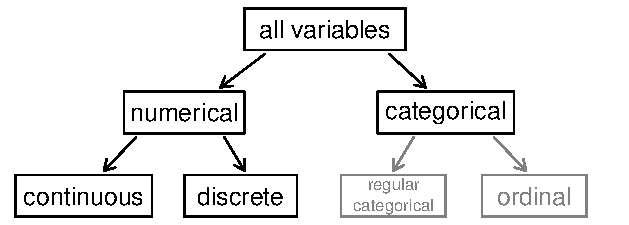
\includegraphics[width=0.57\textwidth]{01/figures/variables/variables}
\caption{Breakdown of variables into their respective types.}
\label{variables}
\end{figure}

Finally, consider the \var{smoking\_ban} variable, which describes the type of county-wide smoking ban and takes values \resp{none}, \resp{partial}, or \resp{comprehensive} in each county. This variable seems to be a hybrid: it is a categorical variable but the levels have a natural ordering. A variable with these properties is called an \term{ordinal} variable. To simplify analyses, any ordinal variables in this book will be treated as categorical variables.

\begin{example}{Data were collected about students in a statistics course. Three variables were recorded for each student: number of siblings, student height, and whether the student had previously taken a statistics course. Classify each of the variables as continuous numerical, discrete numerical, or categorical.}
The number of siblings and student height represent numerical variables. Because the number of siblings is a count, it is discrete. Height varies continuously, so it is a continuous numerical variable. The last variable classifies students into two categories -- those who have and those who have not taken a statistics course -- which makes this variable categorical.
\end{example}

\begin{exercise} \index{data!stroke}
In the stent study from Section~\ref{basicExampleOfStentsAndStrokes}, there were two variables: \var{group} and \var{outcome}. Are these numerical or categorical variables? Answers in the footnote\footnote{There are only two possible values for each variable, and in both cases they describe categories. Thus, each are categorical variables.}.
\end{exercise}

%\begin{example}{What are the variable types of \var{sex} and \var{headL} in the \data{possum} data set?}
%Because the \var{sex} variable takes non-numerical values, it is a categorical variable. Because \var{headL} has numbers as a response and it is meaningful to order these observations by their numbers, it is a numerical variable. More specifically, since \var{headL} can be any length, this variable is a \emph{continuous} numerical variable even though the measured values are all rounded to one decimal.
%\end{example}

%\begin{exercise}
%Identify each of the remaining variables in the \data{possum} data set as either continuous numerical, discrete numerical, or categorical.
%\end{exercise}

%\begin{exercise}\label{possumSiteExer}
%An additional variable was recorded for the \data{possum} data set called \var{site}. Each possum's site is represented a number \resp{1}, \resp{2}, ..., or \resp{7}, however, the ordering of the numbers doesn't actually hold meaning. Is this a numerical or categorical variable? Answer in the footnote\footnote{Because the order of the numbers holds no meaning, this is a categorical variable.}.
%\end{exercise}

\subsection{Relationships between variables}
\label{variableRelations}

%\setlength{\captionwidth}{99mm}
%\begin{figure}
%\begin{center}
%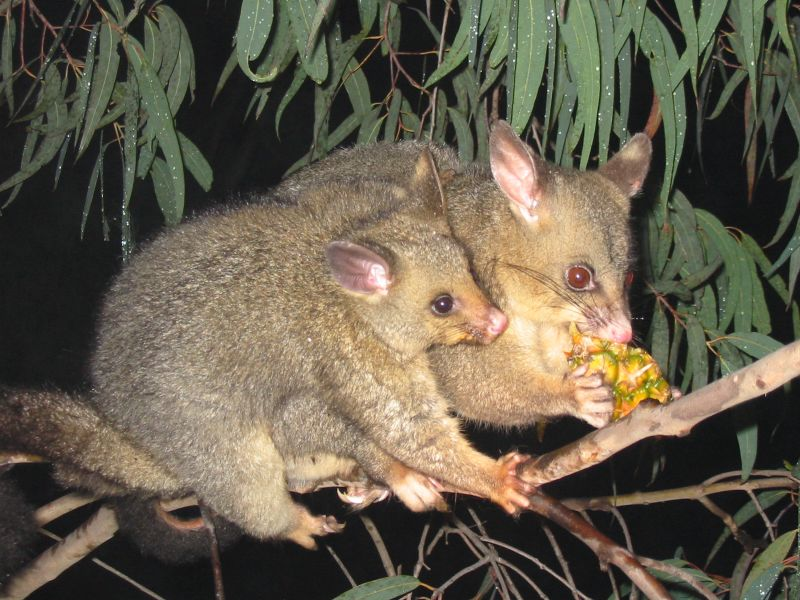
\includegraphics[width=95mm]{01/figures/possumPic/possumPic.jpg} \\
%\addvspace{2mm}
%\begin{minipage}{\textwidth}
%   \caption[possums]{The common brushtail possum of Australia.\vspace{-1mm} \\
%   -----------------------------\vspace{-2mm}\\
%   {\footnotesize Photo by wollombi on Flickr: \urlwofont{http://flickr.com/photos/wollombi/58499575/}}\vspace{-8mm}}
%   \label{possumPic}
%\end{minipage}
%\vspace{3mm}
%\end{center}
%\end{figure}
%\setlength{\captionwidth}{\mycaptionwidth}

Many analyses are motivated by a researcher looking for a relationship between two or more variables. A social scientist may like to know answers to some of the following questions.
\begin{enumerate}
\setlength{\itemsep}{0mm}
%\item[(1)]\label{questionAboutPossumHeadLengthAndWidth} \label{} If a possum has a shorter-than-average head, will its skull width usually be smaller or larger than the average skull width? \label{possumHeadSizeQuestion}
%\item[(2)]\label{maleOrFemalePossumsLonger} Will males or females, on average, be longer? \label{possibleCausationQuestionForPossums}
%\item[(3)]\label{whichPopulationOfPossumWillBeLargerOnAverage} Which population of possums will be larger on average: those living in Victoria or in other locations?
%\item[(4)]\label{doesTheProportionOfMalesDifferBasedOnLocation} Does the proportion of males differ based on location, i.e. from Victoria to the other locations?
\item[(1)]\label{fedSpendingPovertyQuestion} Is federal spending, on average, higher or lower in counties with high rates of poverty?
\item[(2)]\label{ownershipMultiUnitQuestion} If homeownership is lower than the average in one county, will the percent of multi-unit structures in that county likely be above or below average?
	%Do counties that have higher poverty rate also tend to have higher federal spending per capita?
	%Do counties who lean Democrat tend to have a higher or lower poverty rate than counties that lean Republican?
\item[(3)]\label{isAverageIncomeAssociatedWithSmokingBans} Which counties have a higher average income: those that enact one or more smoking bans or those that do not?
%\item[(4)]\label{doesTheProportionOfDemCountiesDifferFromNYToCA} Does the fraction of counties who lean Democrat in two large states, say New York and California, differ?
\end{enumerate}

To answer these questions, data must be collected, such as the \data{county} data set shown in Table~\ref{countyDF}. Examining \termsub{summary statistics}{summary statistic} could provide insights to each of the four questions about counties. Additionally, graphs can be used to visually summarize data and are useful for answering such questions as well.

%\begin{exercise} \label{4possumQuestions}
%Guess what the answer might be to each of the four questions above without examining the data.
%\end{exercise}

%\begin{exercise}
%How confident are you about your answers in Exercise~\exer{4possumQuestions}?
%\end{exercise}

\indexthis{Scatterplots}{scatterplot} are one type of graph used to study the relationship between two numerical variables. Figure~\ref{fed_spendVsPoverty} compares the variables \var{fed\_spend} and \var{poverty}. Each point on the plot represents a single county. For instance, the highlighted dot corresponds to County~1088 in the \data{county} data set: Owsley County, Kentucky, which had a poverty rate of 41.5\% and federal spending of \$21.50 per capita. The scatterplot suggests a slight relationship between the two variables: counties with a high poverty rate also tend to have slightly more federal spending. We might brainstorm as to why this relationship exists and investigate each idea to determine which is the most reasonable explanation.
%, possibly due to national anti-poverty efforts.
\begin{figure}
\centering
\includegraphics[width=0.8\textwidth]{01/figures/fed_spendVsPoverty/fed_spendVsPoverty}
\caption{A scatterplot showing \var{fed\_spend} against \var{poverty}. Owsley County of Kentucky, with a poverty rate of 41.5\% and federal spending of \$21.50 per capita, is highlighted.}
\label{fed_spendVsPoverty}
\end{figure}

\begin{exercise}
Examine the variables in the \data{email50} data set, which are described in Table~\ref{emailVariables} on page~\pageref{emailVariables}. Create two questions about the relationships between these variables that are of interest to you. Two sample questions are in the footnote\footnote{(1) Intuition suggests that if there are many lines in an email then there would tend to also be many characters: does this hold true? (2)~Is there a connection between whether an email is plain text (versus HTML) and whether it is a spam message?}.
\end{exercise}

%\subsection{Associated and independent variables}
%\label{associatedAndIndependentVariablesSubsection}

The \var{fed\_spend} and \var{poverty} variables are said to be associated because the plot shows a discernible pattern. When two variables show some connection with one another, they are called \term{associated} variables. Associated variables can also be called \term{dependent} variables and vice-versa.

\begin{example}{This example examines the relationship between homeownership and the percent of units in multi-unit structures (e.g. apartments, condos), which presented using a scatterplot in Figure~\ref{multiunitsVsOwnership}. Are these variables associated?}
It appears that the larger the fraction of units in multi-unit structures, the lower the homeownership rate. Since there is some relationship between the variables, they are associated.
\end{example}
\begin{figure}
   \centering
   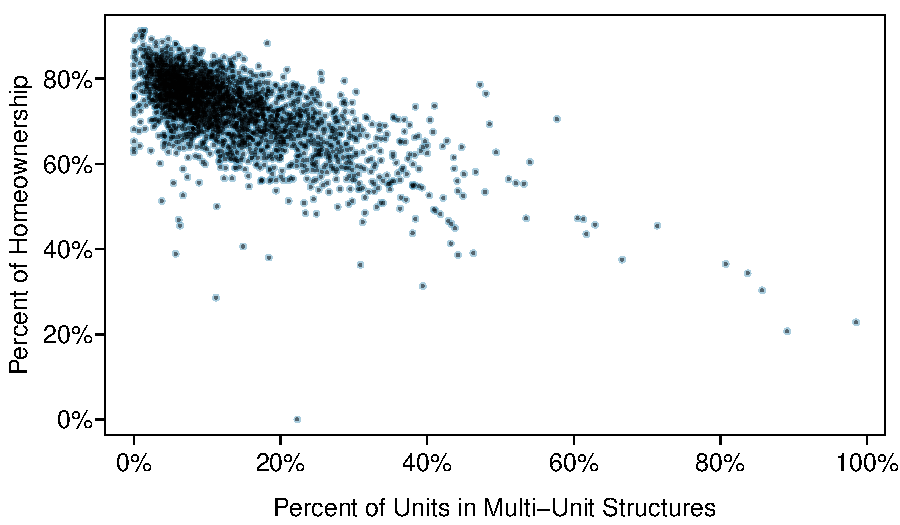
\includegraphics[width=0.8\textwidth]{01/figures/multiunitsVsOwnership/multiunitsVsOwnership}
   \caption{A scatterplot of home ownership versus the percent of units that are in multi-unit structures for all 3,143 counties.}
   \label{multiunitsVsOwnership}
\end{figure}

Because there is a downward trend in Figure~\ref{multiunitsVsOwnership} -- counties with more units in multi-unit structures are associated with lower homeownership -- these variables are said to be \termsub{negatively associated}{negative association}. A \term{positive association} is shown in the relationship between the \var{poverty} and \var{fed\_spend} variables represented in Figure~\ref{fed_spendVsPoverty}, where counties with higher poverty rates tend to receive more federal spending per capita.

If two variables are not associated, then they are said to be \term{independent}. That is, two variables are independent if there is no evident connection between the two.
%It is also possible for cases -- such as a pair of people -- to be independent. For instance, if we select two people randomly from the population, then they are said to be independent.
%It is also possible for cases -- such as a pair of possums or a pair of people -- to be independent. For instance, if possums 1 and 2 are not siblings, do not compete for resources in the same territory, and show no other natural connections, then they can be called independent.
%It is also possible for cases to be independent. Thinking back to the \data{email} data set, two emails with no natural connection  be called independent.

\begin{termBox}{\tBoxTitle{Associated or independent, not both}
A pair of variables are either related in some way (associated) or not (independent). No pair of variables is both associated and independent.}
\end{termBox}

\index{data!county|)}

%%%%%
\section{Overview of data collection principles}
\label{overviewOfDataCollectionPrinciples}

\index{sample|(}
\index{population|(}

The first step in conducting research is to identify topics or questions that are to be investigated. A clearly laid out research question is helpful in identifying what subjects or cases are to be studied and what variables are important. This information provides a foundation for \emph{what} data will be helpful. It is also important that we consider \emph{how} data are collected so that they are trustworthy and help achieve the research goals. %Researchers can be actively engaged in studies called experiments, or they can observe behaviors and collect data in a more passive framework through observational studies. We consider observational studies and data collection methods in this section and then address experiments in Section~\ref{experimentsSection}.

\subsection{Populations and samples}
\label{populationsAndSamples}

Consider the following three research questions:
\begin{enumerate}
\setlength{\itemsep}{0mm}
\item What is the average mercury content in swordfish in the Atlantic Ocean?
\item\label{timeToGraduationQuestionForUCLAStudents} Over the last 5 years, what is the average time to degree for Duke undergraduate students?
\item\label{identifyPopulationOfStentStudy} Does a new drug reduce the number of deaths in patients with severe heart disease?
\end{enumerate}
In each research question, some population of cases is considered. In the first question, all swordfish in the Atlantic ocean are relevant to answering the question. Each fish represents a case, and all of these fish represent the \term{population} of cases. Often times, it is too expensive to collect data for every case in a population. Instead a sample is taken. A \term{sample} represents a subset of the cases and is often a small fraction of the population. For instance, 60 swordfish (or some other number) in the population might be selected, and this sample data may be used to provide an estimate of the population average and answer the research question.

\begin{exercise} \label{identifyingThePopulationForTwoQuestionsInPopAndSampSubsection}
For the second and third questions above, identify what is an individual case and also the population under consideration. Answers in the footnote\footnote{(\ref{timeToGraduationQuestionForUCLAStudents}) Notice that the first question is only relevant to students who complete their degree; the average cannot be computed using a student who never finished her degree. Thus, only Duke undergraduate students who have graduated in the last five years represent cases in the population under consideration. (\ref{identifyPopulationOfStentStudy}) A person with severe heart disease represents a case. The population represents all people with severe heart disease.}.
\end{exercise}


\subsection{Anecdotal evidence}

Consider the following possible responses to our three research questions:
\begin{enumerate}
\item A man on the news got mercury poisoning from eating swordfish, so the average mercury concentration in swordfish must be dangerously high.
\item\label{iKnowThreeStudentsWhoTookMoreThan10YearsToGraduateAtUCLA} I met two students who took more than 10 years to graduate from Duke, so it must take longer to graduate at Duke than at many other colleges.
\item\label{myFriendsDadDiedAfterSulphinpyrazon} My friend's dad had a heart attack and died after they gave him a new heart disease drug, so the drug must not work.
\end{enumerate}
Each of the conclusions are based on some data. However, there are two problems. First, the data only represent one or two cases. Second and more importantly, it is unclear whether these cases are actually representative of the population. Data collected in this haphazard fashion are called \term{anecdotal evidence}.
\setlength{\captionwidth}{\textwidth-80mm}
\begin{figure}
\begin{centering}
\hspace{8mm}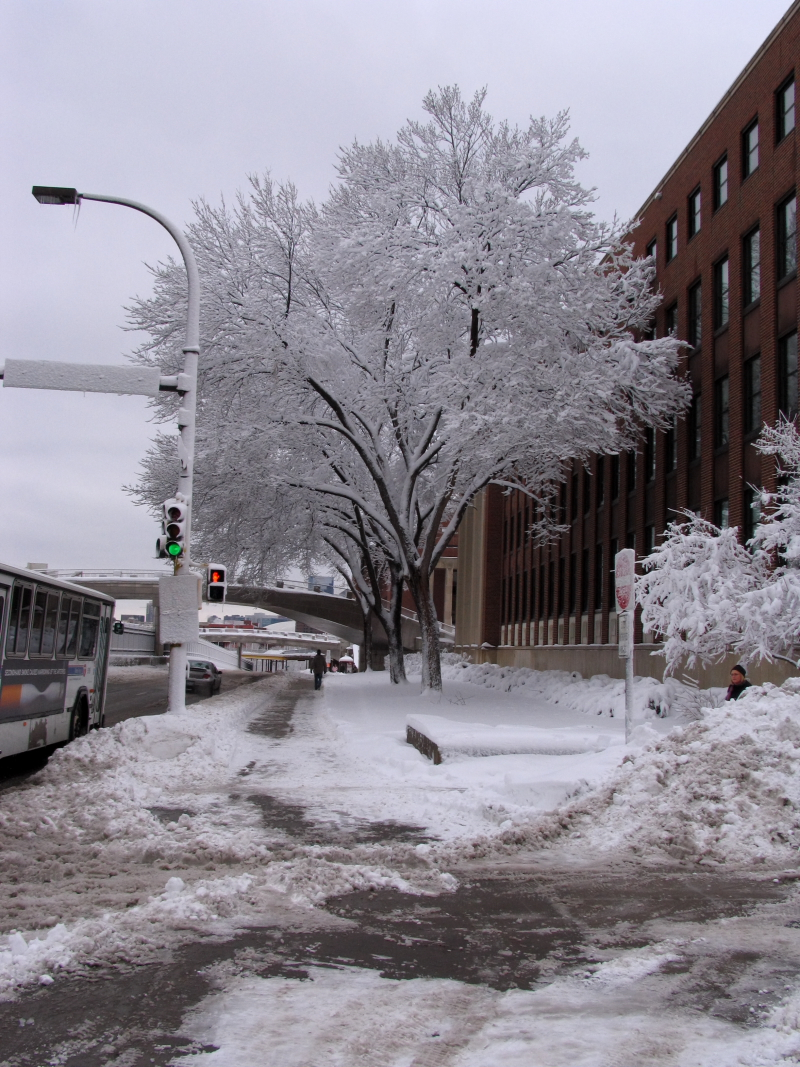
\includegraphics[width=55mm]{01/figures/mnWinter/mnWinter}\hspace{4mm}
\begin{minipage}[b]{\textwidth - 80mm}
   \caption[anecdotal evidence]{In February 2010, some media pundits cited one large snow storm as valid evidence against global warming. As comedian Jon Stewart pointed out, ``It's one storm, in one region, of one country.''\vspace{-4.5mm} \\
   
   -----------------------------\vspace{-2mm}\\
   {\footnotesize February 10th, 2010.}
   \label{mnWinter}}
\end{minipage}
\end{centering}
\end{figure}
\setlength{\captionwidth}{\mycaptionwidth}

\begin{termBox}{\tBoxTitle{Anecdotal evidence}
Data collected in a haphazard fashion. Such evidence may be true and verifiable but often times represents extraordinary cases.}
\end{termBox}

Anecdotal evidence typically is composed of unusual cases that we recall based on their striking characteristics. For instance, we are more likely to remember the two folks we met who took 10 years to graduate than the six others who graduated in four years. Instead of looking at the most unusual cases, we should examine a sample of many cases that represent the population.

\subsection{Sampling from a population}

\index{sample!random sample|(}

We might try to estimate the time to graduate for Duke undergraduates in the last 5 years by collecting a sample of students. All graduates in the last 5 years represent the \emph{population}, and graduates who are selected for review are collectively called the \emph{sample}. In general, we will always seek to \emph{randomly} select a sample from a population. The most basic type of random selection is equivalent to how raffles are run. For example, in selecting graduates, we could write each graduate's name on a raffle ticket and draw 100 tickets. The selected names would represent a random sample of 100 graduates.
\begin{figure}[ht]
\centering
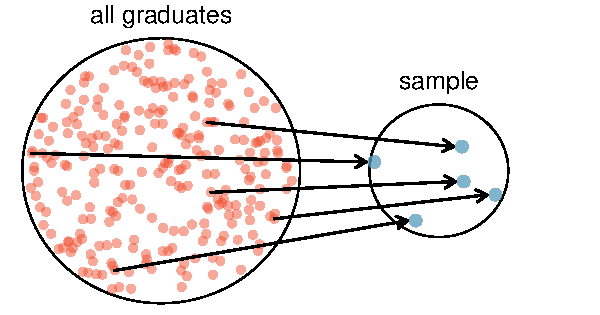
\includegraphics[height=1.5in]{01/figures/popToSample/popToSampleGraduates}
\caption{In this graphic, five graduates are randomly selected from the population to be included in the sample.}
\label{popToSampleGraduates}
\end{figure}

Why pick a sample randomly? Why not just pick a sample by hand? Consider the following scenario.

\begin{exercise}
Suppose we ask a student who happens to be majoring in nutrition to select several graduates for the study. What kind of students do you think she might collect? Do you think her sample would be representative of all graduates? Comment in the footnote\footnote{We really don't know. Perhaps she would pick a disproportionate number of graduates from health-related fields. Or perhaps her selection would be well-representative of the population. When selecting samples by hand, we run the risk of picking a \emph{biased} sample, even if that bias is unintentional or difficult to discern.}.
\end{exercise}
\begin{figure}
\centering
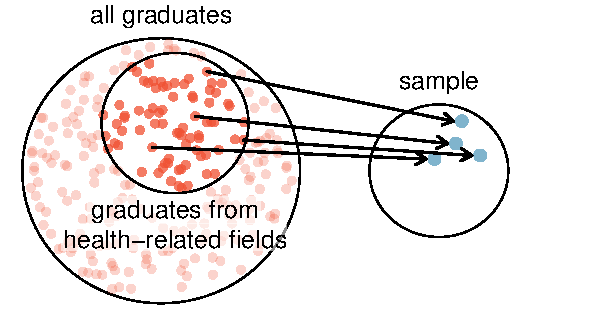
\includegraphics[height=1.5in]{01/figures/popToSample/popToSubSampleGraduates}
\caption{Instead of sampling from all graduates equally, a nutrition major might inadvertently pick graduates with health-related majors disproportionally often.}
\label{popToSubSampleGraduates}
\end{figure}

If someone was permitted to pick and choose exactly which graduates were included in the sample, it is entirely possible that the sample could be skewed to that person's interests, which may be entirely unintentional. This introduces \term{bias} into a sample. Sampling randomly helps resolve this problem. The most basic random sample is called a \term{simple random sample}, and it is the equivalent of using a raffle to select cases. This means that each case in the population has an equal chance of being included and there is no implied connection between the cases in the sample. The act of taking a simple random sample helps eliminate bias, however, bias can still crop up in other ways.

Even when people are %seemingly 
picked at random (for surveys, etc.), caution must be exercised if the \term{non-response} \index{sample!non-response|textbf} is high. For instance, if only 30\% of the people randomly sampled for a survey actually respond, then it is unclear whether the results are \term{representative} of the entire population. This \term{non-response bias} \index{sample!non-response bias|textbf} can skew results.
\begin{figure}[h]
\centering
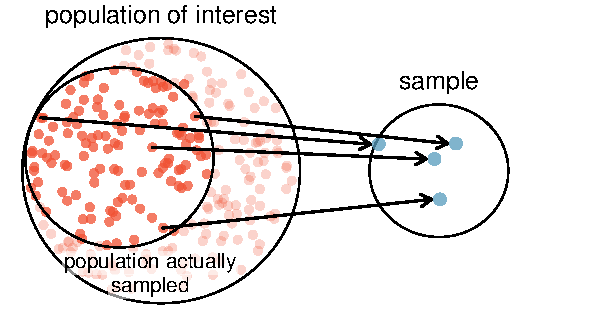
\includegraphics[height=1.5in]{01/figures/popToSample/surveySample}
\caption{Surveys may result in only reaching a certain group within the population, and it is not easy, and often times impossible, to fix this problem.}
\label{surveySample}
\end{figure}

Another common downfall is a \term{convenience sample}\index{sample!convenience sample}, where individuals who are easily accessible are more likely to be included in the sample. For instance, if a political survey is done by stopping people walking in the Bronx, this will not represent all of New York City. It is often difficult to discern what sub-population a convenience sample represents.

\begin{exercise}
We can easily access ratings for products, sellers, and companies through websites. These ratings are based only on those people who go out of their way to provide a rating. If 50\% of online reviews for a product are negative, do you think this means that 50\% of buyers are dissatisfied with the product? Our thoughts are provided in the footnote\footnote{From our own (anecdotal!) experiences, we believe people tend to rant more about products that fell below expectations than rave about those products that perform as expected. For this reason, we suspect there is a negative bias in product ratings on sites like Amazon. However, since our experiences may not be representative, we also keep an open mind should data on the subject become available.}.
\end{exercise}

\index{sample!random sample|)}
\index{population|)}
\index{sample|)}

\subsection{Explanatory and response variables}
\label{explanatoryAndResponse}

\index{data!county|(}

Consider the following question from page~\pageref{fedSpendingPovertyQuestion} for the \data{county} data set:
\begin{enumerate}
\item[(1)] 
	Is federal spending, on average, higher or lower in counties with high rates of poverty?
%Will males or females, on the average, be longer?
\end{enumerate}
This question might be motivated by the belief that some aims of federal spending are to reduce areas of high poverty. If we suspect poverty might affect spending in a county, then \var{poverty} is the \term{explanatory} variable and \var{fed\_spend} is the \term{response} variable in the relationship\footnote{Sometimes the explanatory variable is called the \term{independent} variable and the response variable is called the \term{dependent} variable. However, this becomes confusing since a \emph{pair} of variables might be independent or dependent, so we avoid this language.}. If there are many variables, it may be possible to label a number of them as explanatory and the others as response variables.

\begin{tipBox}{\tipBoxTitle{Explanatory and response variables}
To identify the explanatory variable in a pair of variables, identify which of the two is suspected of affecting the other.

\hspace{10mm}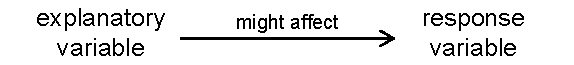
\includegraphics[height=0.34in]{01/figures/expResp/expResp}}
\end{tipBox}

\begin{caution}{association does not imply causation}{Labeling variables as \emph{explanatory} and \emph{response} does not guarantee the relationship between the two is actually causal, even if there is an association identified between the two variables. We use these labels only to keep track of which variable we suspect affects the other.}
\end{caution}

In some cases, there is no explanatory or response variable. Consider the following question from page~\pageref{ownershipMultiUnitQuestion}:
\begin{enumerate}
\item[(2)] 
	If homeownership is lower than the average in one county, will the percent of multi-unit structures in that county likely be above or below average?
\end{enumerate}
It is especially difficult to decide which of these variables should be considered the explanatory and response variable, %there does not have an explanatory variable since it is unclear whether \var{homeownership} would affect \var{multiunit} or vice-versa, 
i.e. the direction is ambiguous, so no explanatory or response labels are suggested here.

\index{data!county|)}

\subsection{Introducing observational studies and experiments}

There are two primary types of data collection: observational studies and experiments.

Researchers perform an \term{observational study} when they collect data in a way that does not directly interfere with how the data arise. For instance, researchers may collect information using surveys, reviewing medical or company records, or follow a \term{cohort} of many similar individuals to consider why certain diseases might develop. In each of these cases, the researchers try not to interfere with the natural order of how the data arise. In general, observational studies can provide evidence of a naturally occurring association between variables, but they cannot show a causal connection.

When researchers want to establish a causal connection, they conduct an \term{experiment}. Usually there will be both an explanatory and a response variable. For instance, we may suspect administering a drug will reduce mortality in heart attack patients over the following year. To check if there really is a causal connection between the explanatory variable and the response, researchers will collect a sample of individuals and split the cases into groups. The cases in each group are \emph{assigned} a treatment. When the groups are created using a randomization technique, the experiment is called a \term{randomized experiment}. For example, each heart attack patient in the drug trial could be randomly assigned (e.g. by flipping a coin) into one of two groups: the first group receives a placebo (fake treatment) and the second group receives the drug. See the case study in Section~\ref{basicExampleOfStentsAndStrokes} for another example of an experiment, though that study did not employ a placebo.

\begin{tipBox}{\tipBoxTitle{association $\neq$ causation}
In general, association does not imply causation, and causation can only be inferred from a randomized experiment.}
\end{tipBox}


%%%%%
\section{Observational studies and sampling strategies}

\subsection{Observational studies}

The \data{county} data set was from an observational study. While the government coordinated with local governments and hundreds of millions of people to collect data, the variables were naturally occurring. Generally, data in observational studies are collected only by monitoring what occurs or intermittent inquiries, while experiments require the primary explanatory variable in a study be assigned for each subject by the researchers.

Inferring causal conclusions from experiments is often reasonable. However, making the same causal conclusions from observational data can be treacherous and is not recommended. Thus, we can generally only infer associations from observational data.

\begin{exercise} \label{sunscreenLurkingExample}
Suppose an observational study tracked sunscreen use and skin cancer, and it was found that the more sunscreen someone used, the more likely the person was to have skin cancer. Does this mean sunscreen \emph{causes} skin cancer?
\end{exercise}

Previous research tells us that using sunscreen actually reduces skin cancer risk, so maybe there is another variable that can explain this hypothetical association between sunscreen usage and skin cancer. One important piece of information absent is sun exposure. If someone is out in the sun all day, she is more likely to use sunscreen \emph{and} more likely to get skin cancer. Exposure to the sun is unaccounted for in the investigation, giving the incorrect impression that sunscreen causes skin cancer.
\begin{center}
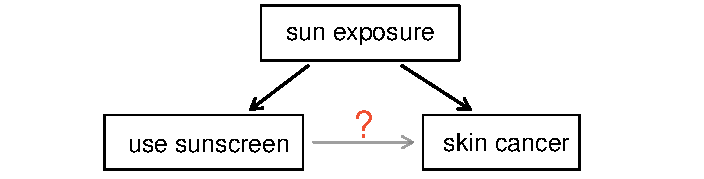
\includegraphics[height=1.0in]{01/figures/variables/sunCausesCancer}
\end{center}
%It just so happens that if someone is exposed to the sun they also usually use sunscreen. 

Sun exposure is what is called a \term{lurking variable}\footnote{Also called a \term{confounding variable}, \term{confounding factor}, or a \term{confounder}.}, which is a variable that is correlated with both the explanatory and response variables. While one method to justify making causal conclusions from observational studies is to exhaust the search for lurking variables, there is no guarantee that all lurking variables can be examined or measured.

In the same way, the \data{county} data set is an observational study with possible lurking variables, and its data cannot easily be used to make causal conclusions.

\begin{exercise}
Figure~\ref{multiunitsVsOwnership} shows a negative association between homeownership rate and the percentage of multi-unit structures in a county. However, it is unreasonable to conclude that there is some causal relationship between the two variables. Suppose a social scientist conjectured, based on Figure~\ref{multiunitsVsOwnership}, that there was a causal connection. Suggest one or more other variables that might explain the relationship we see. One explanation is provided in the footnote\footnote{Population density may be important. If a county is very dense, then this may require a larger fraction of residents to live in multi-unit structures. Additionally, the high density may contribute to increases in property value, making homeownership infeasible for many residents.}.
% in the proportion of possums that are male based on location. However, it is unreasonable to conclude that this is a causal relationship because the data are observational. Suggest at least one lurking variable that might be the true cause for the differences in \var{sex}. One possibility is listed in the footnote\footnote{Some genes can affect one gender more than the other. If the \resp{other} population has a gene that affects males more positively than females and this gene is less common in the \resp{Vic} population, this might explain the difference in gender ratio for each level of \var{pop}.}.
\end{exercise}

Observational studies come in two forms: prospective and retrospective studies. A \term{prospective study} identifies individuals and collects information as events unfold. For instance, medical researchers may identify and follow a group of similar individuals over many years to assess the possible influences of behavior on cancer risk. \termsub{Retrospective studies}{retrospective studies} collect data after events have taken place, e.g. researchers may review past events in medical records. Some data sets, such as \data{county}, may contain both prospectively- and retrospectively-collected variables. Local governments prospectively collected some variables as events unfolded (e.g. retails sales) while the federal government retrospectively collected others during the 2010 census (e.g. county population counts). %The \data{county} data are an example of a retrospective study.

\subsection{Three sampling methods (special topic)}
\label{threeSamplingMethods}

Almost all statistical methods are based on the notion of implied randomness. If observational data are not collected in a random framework from a population, these statistical methods -- the estimates and computed errors -- are not reliable. Here we consider three random sampling techniques: simple, stratified, and cluster sampling.

\termsub{Simple random sampling}{sample!simple random sampling} is probably the most intuitive form of random sampling. Consider the salaries of Major League Baseball (MLB) players, where each player is a member of one of the league's 30 teams. To take a simple random sample of 120 baseball players and their salaries from the 2010 season, we could write the names of that season's 828 players onto ping pong balls, drop the ping pong balls into a bucket, shake the bucket around until we are sure it's all mixed up, then draw out balls from the bucket until we have the sample of 120 players. In general, a sample is referred to as ``simple random'' if each case in the population has an equal chance of being included in the final sample \emph{and} knowing that a case is included in a sample does not provide useful information about which other cases/outcomes are included.

\termsub{Stratified sampling}{sample!stratified sampling} is a divide-and-conquer sampling strategy. The population is divided up into groups called \term{strata} \index{sample!strata|textbf} where the strata are chosen so that similar cases are grouped, then a second sampling method (such as simple random sampling) is employed within each stratum. In the baseball salary example, the teams could represent the strata; some teams have much more money (we're looking at you, Yankees). Then we might randomly sample four players from each team for a total of 120 players.

Stratified sampling is especially useful when the cases in each stratum are very similar in the measured outcome. For instance, the baseball teams might be useful strata since some teams have (much) more money and therefore tend to pay players more. The downside is that analyzing data from a stratified sample is more complex than analyzing data from a simple random sample, and the analysis methods introduced in this book would need to be extended.

\begin{example}{Why would it be good for cases within each stratum to be very similar?}
We might get a more stable statistical estimate for the subpopulation in a stratum if the cases are very similar. Then when we summarize the entire population, these individual stable estimates for each subpopulation will help us build a reliable estimate for the full population.
\end{example}

A \termsub{cluster sample}{sample!cluster sample} is much like a two-stage simple random sample. We break up the population into many groups, called \termsub{clusters}{sample!cluster}. Then we sample a fixed number of clusters and collect a simple random sample in each cluster. This technique is similar to stratified sampling in its process, except that there is no requirement to sample from every cluster while stratified sampling requires observations from every stratum.
\begin{figure}
\centering
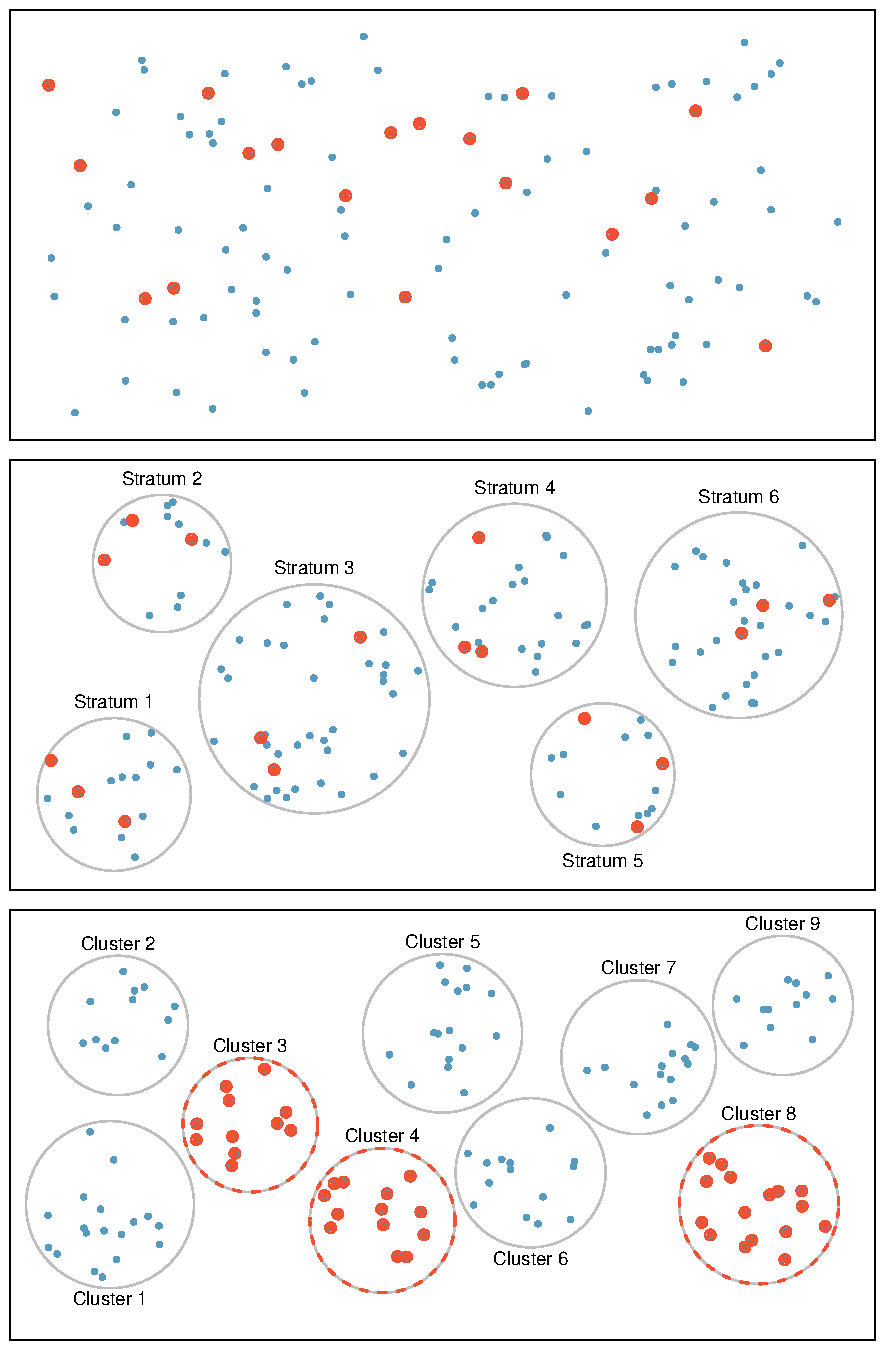
\includegraphics[width=0.8\textwidth]{01/figures/samplingMethodsFigure/samplingMethodsFigure}
\caption{Examples of simple random, stratified, and cluster sampling. In the top panel, simple random sampling was used to randomly select the 18 cases. In the middle panel, stratified sampling was used: cases were grouped into strata, and then simple random sampling was employed within each stratum. In the bottom panel, cluster sampling was used, where data were binned into nine clusters, three of the clusters were randomly selected, and six cases were randomly sampled in each of these clusters.}
\label{samplingMethodsFigure}
\end{figure}

Sometimes cluster sampling can be a more economical random sampling technique than alternatives. Also, unlike stratified sampling, cluster sampling is most helpful when there is a lot of case-to-case variability within a cluster but the clusters themselves don't look very different from one another (e.g. if neighborhoods represented clusters, then it is best if each neighborhood is very diverse). A downside of cluster sampling is that more advanced analysis techniques are typically required, though the methods in this book can be extended to handle such data.

\begin{example}{Describe a scenario where cluster sampling would be much easier than simple random or stratified sampling.}
Suppose we are interested in estimating the malaria rate in a densely tropical portion of rural Indonesia. We learn that there are 30 villages in that part of the Indonesian jungle, each more or less similar to the next. Our goal is to test 150 individuals for malaria. In this case, a simple random sample would likely draw individuals from all 30 villages, which could make data collection extremely expensive. Stratified sampling would be a challenge since it is unclear how we would build stratum of similar individuals. However, cluster sampling seems like a very good idea. First, we might randomly select half the villages, then randomly select 10 people from each. This would probably reduce our data collection costs substantially in comparison to a simple random sample and would still give us reliable information.

%Suppose we were sampling tree circumferences in a large forest. It is unclear how we might randomly sample individual trees -- and even if we could, it would be a substantial trek to reach each individual tree in the sample. While it seems possible to build up strata, perhaps using regions in the forest, it is still unclear how we should sample the trees in each stratum. If there are only a small number of strata, we run into the same trouble as in simple random sampling. Additionally, the strata are probably not terribly uniform; tree sizes often vary quite a bit, even in a small region.  If there are many strata, then we must travel far and wide to reach each of them.

%A cluster sample would be much easier to employ, and there are a number of possible cluster sampling strategies -- we present one. We could first divide up the forest into a grid of squares that are 10 meters on each side\footnote{One possible objection: we also must be able to find the precise locations in the forest when we collect data. However, a GPS device could resolve this concern.}. Each of these grid regions could represent a cluster. Next we could randomly sample the clusters where we would actually take tree measurements. For each selected cluster, we might just conduct an exhaustive sample, measuring the circumference of all the trees in that cluster.
\end{example}

%\begin{exercise}
%Describe a second situation where cluster sampling would be more convenient than simple random or stratified sampling. See the footnote for another example\footnote{Describe another example...}.
%\end{exercise}


%%%%%
\section{Experiments}
\label{experimentsSection}

Studies where the researchers assign treatments to cases are called \termsub{experiments}{experiment}. When cases are randomly assigned to the treatment groups, it is called a \term{randomized experiment}. Randomized experiments are fundamentally important when trying to show a causal connection between two variables.

\subsection{Principles of experimental design}
\label{experimentalDesignPrinciples}

Randomized experiments are generally built on four principles.
\begin{description}
\item[Controlling.] Researchers assign treatments to cases, and they do their best to \term{control} any other differences in the groups. For instance, if a drug treatment in the form of a pill may be affected by how much water a patient drinks with the drug, the doctor may ask all patients to drink a 12 ounce glass of water with the pill to reduce one source of unnecessary variability between the cases.
\item[Randomization.] Researchers randomize patients into the groups to account for variables that cannot be controlled. In a clinical trial, some patients may be more susceptible to a disease than others due to their genetic make-up. Randomizing patients into the two treatment groups is one way to help even out the genetic differences in each group, and it also prevents accidental bias from entering the study.
\item[Replication.] The more cases researchers observe, the more accurately they can estimate the effect of the explanatory variable on the response. In a single study, we \term{replicate} by collecting a sufficiently large sample. Additionally, a group of scientists may replicate an entire study to verify an earlier finding.
\begin{figure}
\centering
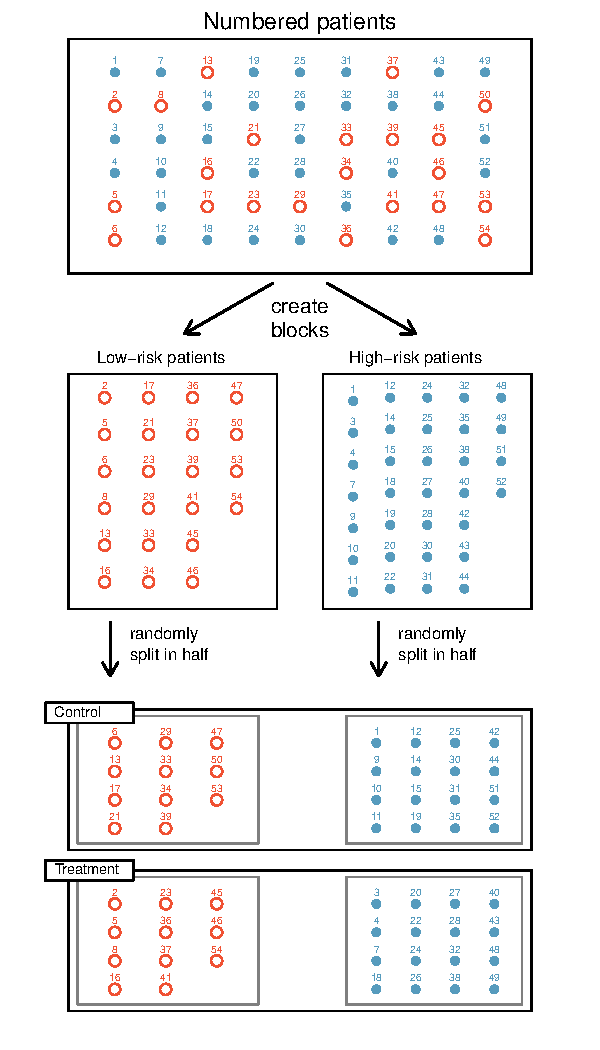
\includegraphics[width=0.78\textwidth]{01/figures/figureShowingBlocking/figureShowingBlocking}
\caption{Blocking using a variable depicting patient risk. Patients are first divided into low-risk and high-risk blocks, then each block is evenly divided into the treatment groups using randomization. This strategy ensures an equal number of patients in each treatment group from both the low-risk and high-risk categories.}
\label{figureShowingBlocking}
\end{figure}
\item[Blocking.] Researchers sometimes know or suspect variables other than the treatment might influence the response. Under these circumstances, they may first group individuals based on this variable into \term{blocks} and then randomize cases within each block to the treatment groups. This strategy is often referred to as \term{blocking}. For instance, if we were looking at the effect of a drug on heart attacks, we might first split patients in the study into low-risk and high-risk blocks, then randomly assigning half the patients from each block to the control group and the other half to the treatment group, as shown in Figure~\ref{figureShowingBlocking}. This strategy ensures each treatment group has an equal number of low-risk and high-risk patients.
\end{description}

It is important to incorporate the first three experimental design principles into any study, and this book describes applicable methods for analyzing data from such experiments. Blocking is a slightly more advanced technique, and statistical methods in this book may be extended to analyze data collected using blocking. \Comment{MAY BE APPROPRIATE TO REVISE THIS SENTENCE IF MORE DISCUSSION AND METHODS ARE ADDED TO CHAPTER 8.}

\subsection{Reducing bias in human experiments}
\label{biasInHumanExperiments}

Randomized experiments are the gold standard for data collection, but they do not ensure an unbiased perspective into the cause and effect relationships in all cases. Human studies are perfect examples where bias can unintentionally arise. Here we reconsider a study where a new drug was used to treat heart attack patients\footnote{Anturane Reinfarction Trial Research Group. 1980. Sulfinpyrazone in the prevention of sudden death after myocardial infarction. New England Journal of Medicine 302(5):250-256.}. In particular, researchers wanted to know if the drug reduced deaths in patients.

These researchers designed a randomized experiment because they wanted to draw causal conclusions about the drug's effect. Study volunteers\footnote{Human subjects are often called \term{patients}, \term{volunteers}, or \term{study participants}.} were randomly placed into two study groups. One group, the \term{treatment group}, received the drug. The other group, called the \term{control group}, did not receive any drug treatment.

Put yourself in the place of a person in the study. If you are in the treatment group, you are given a fancy new drug that you anticipate will help you. On the other hand, a person in the other group doesn't receive the drug and sits idly, hoping her participation doesn't increase her risk of death. These perspectives suggest there are actually two effects: the one of interest is the effectiveness of the drug and the second is an emotional effect that is difficult to quantify.

Researchers aren't interested in this emotional effect, which might bias the study. To circumvent this problem, researchers do not want patients to know which group they are in. When researchers keep the patients uninformed about their treatment, the study is said to be \term{blind}. But there is one problem: if a patient doesn't receive a treatment, she will know she is in the control group. The solution to this problem is to give fake treatments to patients in the control group. A fake treatment is called a \term{placebo}, and an effective placebo is the key to making a study truly blind. A classic example of a placebo is a sugar pill that is made to look like the actual treatment pill. Often times, a placebo results in a slight but real improvement in patients. This often positive effect has been dubbed the \term{placebo effect}.

The patients are not the only ones who should be blinded: doctors and researchers can accidentally bias a study. When a doctor knows a patient has been given the real treatment, she might inadvertently give that patient more attention or care than a patient that she knows is on the placebo. To guard against this bias (which again has been found to have a measurable effect in some instances), most modern studies employ a \term{double-blind} setup where doctors or researchers who interact with patients are, just like the patients, unaware of who is or is not receiving the treatment\footnote{There are always some researchers involved in the study who do know which patients are receiving which treatment. However, they do not have interactions with the patients and do not tell the blinded doctors who is receiving which treatment.}.

\begin{exercise}
Look back to the study in Section~\ref{basicExampleOfStentsAndStrokes} where researchers were testing whether stents were effective at reducing strokes in at-risk patients. Is this an experiment? Was the study blinded? Was it double-blinded? Answers in the footnote\footnote{The researchers assigned the patients into their treatment groups, so this study was an experiment. However, the patients could distinguish what treatment they received, so this study was not blind. The study could not be double-blind since it was not blind.}.
\end{exercise}


%%%%%
\section{Examining numerical data}
\label{numericalData}

We explore several graphical and summary techniques in this section for numerical variables using the \data{email50} and \data{county} data sets discussed in Section~\ref{dataBasics}. Recall that numerical variables include only outcomes that are numbers and where it is reasonable to perform basic arithmetic with those numbers. For example, \var{pop2010} is a numerical variable since we can sensibly discuss the difference or ratio of the population in two counties. On the other hand, area codes and zip codes are not numerical variables, rather they are~categorical.

%This larger set of cases is called the \term{population}. Ideally data would be collected from every case in the population. However, this is rarely possible due to high costs of data collection. As a substitute, statisticians collect subsets of the data called \termsub{samples}{sample} to gain insights into the population. The \data{cars} data set represents a sample of all cars from 1993, and the \data{possum} data set represents a sample from all possums in the Australian states of Victoria, New South Wales, and Queensland. In this section we introduce summary statistics and graphics as a first step in analyzing numerical data from a sample to help us understand certain features of the population as a whole.

\subsection{Scatterplots for paired data}
\label{scatterPlots}

\index{data!email50|(}

A \term{scatterplot} provides a case-by-case view of data for two numerical variables. In Section~\ref{variableRelations} on page~\pageref{fed_spendVsPoverty}, a scatterplot was used to examine how federal spending and poverty were related in the \data{county} data set. Another scatterplot is shown in Figure~\ref{email50LinesCharacters}, comparing \var{lines} (number of lines) and \var{num\_char} (number of characters) in emails for the \data{email50} data set.
\begin{figure}[h]
   \centering
   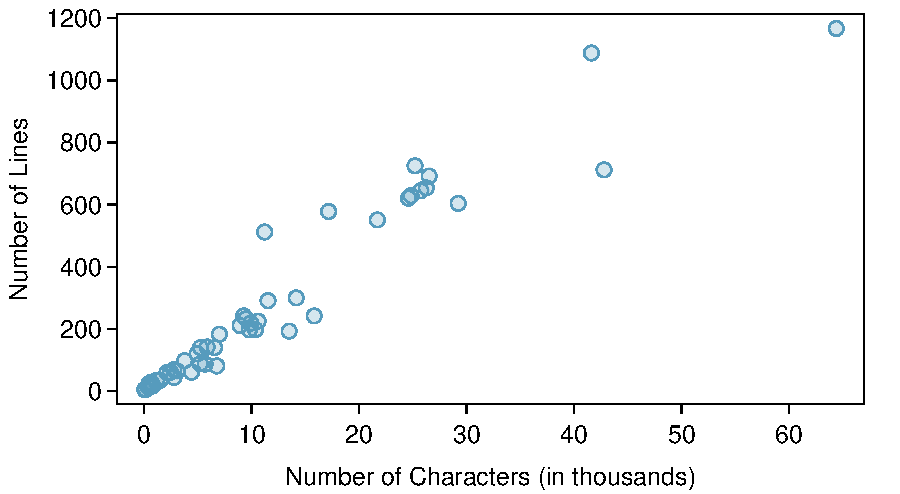
\includegraphics[width=0.75\textwidth]{01/figures/email50LinesCharacters/email50LinesCharacters} %carsPriceVsWeight/carsPriceVsWeight}
   \caption{A scatterplot of \var{lines} versus \var{num\_char} for the \data{email50} data.}
   \label{email50LinesCharacters} %carsPriceVsWeight}
\end{figure}

In any scatterplot, each point represents a single case. Since there are 50 cases in \data{email50}, there are 50 points in Figure~\ref{email50LinesCharacters}.

\begin{exercise}
What do scatterplots reveal about the data, and how might they be useful? One answer is provided in the footnote\footnote{Scatterplots are helpful in quickly spotting associations relating variables, whether those associations come in the form of simple trends or whether those relationships are more complex.} % The simple scatterplot is an exceptional tools for inspiration and insight into the relationship between two variables.}.
\end{exercise}

\begin{example}{Some associations are more linear, like the relationship between \var{fed\_spend} and \var{poverty} shown in Figure~\ref{fed_spendVsPoverty} on page~\pageref{fed_spendVsPoverty} and the plot shown above in Figure~\ref{email50LinesCharacters}. Others can be \emph{nonlinear}. In this example we consider a new data set of 54 cars with two variables: vehicle price and~weight\footnote{Source: \url{http://www.amstat.org/publications/jse/v1n1/datasets.lock.html}}.}
A scatterplot of vehicle price versus weight is shown in Figure~\ref{carsPriceVsWeight}. Notice the curved trend in the data. Investigation of nonlinearity is sometimes critical in a data analysis.
\begin{figure}[h]
   \centering
   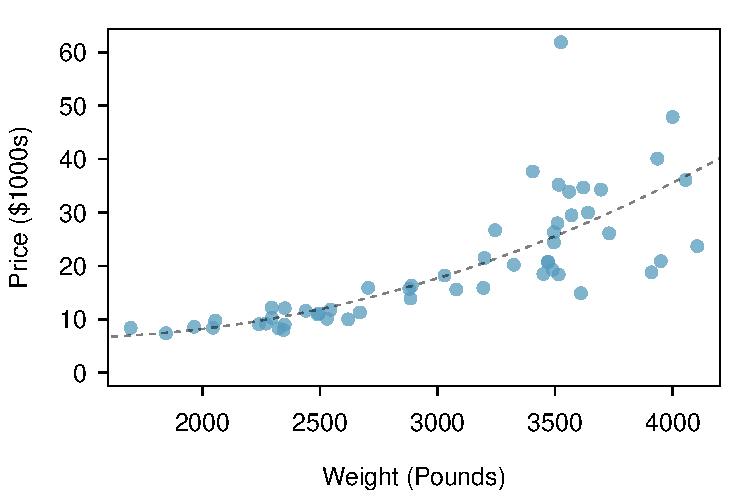
\includegraphics[width=0.65\textwidth]{01/figures/carsPriceVsWeight/carsPriceVsWeight}
   \caption{A scatterplot of \var{price} versus \var{weight} for 54 cars.}
   \label{carsPriceVsWeight}
\end{figure}
\end{example}

\begin{exercise}
Describe two variables that would have a horseshoe shaped association in a scatterplot. One example is given in the footnote\footnote{Consider the case where your vertical axis represents something ``good'' and your horizontal axis represents something that is only good in moderation. Health and water consumption fit this description since water becomes toxic when consumed in excessive quantities.}.
\end{exercise}

\subsection{Dot plots and the mean}
\label{dotPlot}

Sometimes two variables is one too many: only one variable may be of interest. In these cases, a dot plot provides the most basic of displays. A~dot plot is a one-variable scatterplot, and a dot plot of the number of characters from 50 emails is shown in Figure~\ref{emailCharactersDotPlot}.
\begin{figure}[h]
   \centering
   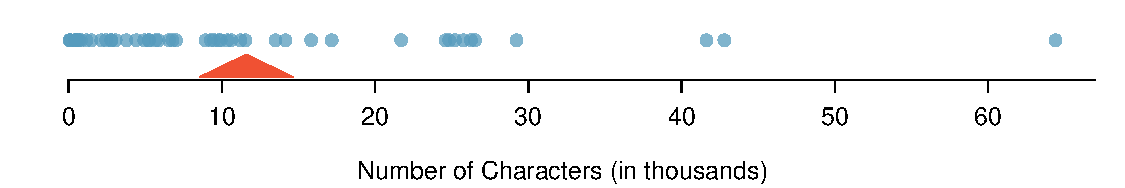
\includegraphics[width=\textwidth]{01/figures/emailCharactersDotPlot/emailCharactersDotPlot} %carsPriceDotPlot/carsPriceDotPlot}
   \caption{A dot plot of \var{num\_char} for the \data{email50} data set. The triangle marks the sample's mean.}
   \label{emailCharactersDotPlot} %carsPriceDotPlot}
\end{figure}

The \term{mean}, sometimes called the \indexthis{average}{mean!average}, is a way to measure the center of a \term{distribution} of data. To find the mean number of characters in the 50 emails, we add up all the character counts and divide by the number of cases:
\begin{eqnarray}
\bar{x} = \frac{963 + 15586 + \cdots + 4371}{50} = 12422
%\bar{x} = \frac{15.9 + 33.9 + \cdots + 26.7}{54} = 19.99259
\label{sampleMeanEquation}
\end{eqnarray}
The sample mean is often labeled $\bar{x}$\marginpar[\raggedright$\bar{x}$\\\footnotesize sample\\ mean]{\raggedright$\bar{x}$\\\footnotesize sample\\ mean}. The letter $x$ is being used as an abbreviation for \var{num\_char}, and the bar says it is the average number of characters in the 50 emails was 12,422. It is useful to think of the mean as the balancing point of the distribution. The sample mean is shown as a blue triangle in Figure~\ref{emailCharactersDotPlot}.

\begin{termBox}{\tBoxTitle{Mean}
The sample mean of a numerical variable is computed as the sum of all of the observations divided by the number of observations:
\begin{eqnarray}
\bar{x} = \frac{x_1+x_2+\cdots+x_n}{n}
\label{meanEquation}
\end{eqnarray}
where $x_1, x_2, \dots, x_n$ represent the $n$ observed values.}
\end{termBox}\marginpar[\raggedright\vspace{-8mm}

$n$\\\footnotesize sample size]{\raggedright\vspace{-8mm}

$n$\\\footnotesize sample size}\vspace{-2mm}

\begin{exercise}
Examine equations~(\ref{sampleMeanEquation}) and~(\ref{meanEquation}) above. What does $x_1$ correspond to? And $x_2$? Can you infer a general meaning to what $x_i$ might represent? Answers in the footnote\footnote{$x_1$ corresponds to the number of characters in the first email in the sample (963), $x_2$ to the number of characters in the second email (15,586), and $x_i$ corresponds to the number of characters in the $i^{th}$ email in the data set.}.
\end{exercise}

\begin{exercise}
What was $n$ in this sample of emails? Answer in the footnote\footnote{The sample size was $n=50$.}.
\end{exercise}

The \data{email50} data set represents a sample from a larger population of emails that were received in January and February. We could compute this population mean in the same way as the sample mean, however, the population mean has a special label: $\mu$. \index{Greek!$\mu$} \index{Greek!mu} The symbol $\mu$\marginpar[\raggedright$\mu$\\\footnotesize population\\ mean]{\raggedright$\mu$\\\footnotesize population\\ mean} is the Greek letter \emph{mu} and represents the average of all observations in the population. Sometimes a subscript, such as $_x$, is used to represent which variable the population mean refers to, i.e. $\mu_x$.

\begin{example}{The average number of characters across all emails can be estimated using the sample data. Based on the sample of 50 emails, what would be a reasonable estimate of $\mu_x$, the mean number of characters in all emails in the \data{email} data set? (Recall that \data{email50} is a sample from \data{email}.)}
The sample mean, 12,422, may provide a reasonable estimate of $\mu_x$. While this estimate will not be perfect, it provides a \emph{point estimate} of the population mean. In Chapter~\ref{foundationsForInference} and beyond, we will develop tools to characterize the accuracy of point estimates, and we will find that point estimates based on larger samples tend to be more accurate than those based on smaller samples.
\end{example}
% Note that the mean in the full email data sets is 625.4, which is substantially influenced by strong skew

\begin{example}{We might like to compute the average income per person in the U.S. To do so, one might first think to take the mean of the per capita incomes across the 3,143 counties in the \data{county} data set. What would be a better approach?} \label{wtdMeanOfIncome}
The \data{county} data set is special in that each county actually represents many individual people. If we were to simply average across the \var{income} variable, we would be treating counties with 5,000 and 5,000,000 residents equally in the calculations. Instead, we should compute the total amount of money made in each county, add up all the counties' totals, and then divide by the number of people in all the counties. %The total amount of money in a county is equal to the per capita income times the number of people:
%\begin{align*}
%\text{money for county }i &= \text{(per capita income) }*\text{ (number of residents)} \\
%			&= income_i*pop2010_i
%\end{align*}
%Above, we have used the variables $income_i$ and $pop2010_i$ to represent the per capita income $i^{th}$
If we completed these steps with the \data{county} data, we would find the per capita income for the U.S. is \$27,348.43. Had we computed the \emph{simple} mean of per capita income across counties, the result would have been just \$22,504.70!
\end{example}

Example~\ref{wtdMeanOfIncome} used what is called a \term{weighted mean}\index{mean!weighted mean}, which will not be a key topic in this textbook. However, we have provided an online supplement on weighted means for interested readers:
\begin{center}
\Comment{CREATE 1-2 PAGE DISCUSSION, PUT LINK HERE}
\end{center}

\subsection{Histograms and shape}
\label{histogramsAndShape}

Dot plots show the exact value for each observation. This is useful for small data sets, but can become problematic for larger samples. Rather than showing the value of each observation, we might prefer to think of the value as belonging to a \emph{bin}. For example, in the \data{email50} data set, we could create a table of counts for the number of cases with character counts between 0 and 5,000, then the number of cases between 5,000 and 10,000, and so on. Observations that fall on the boundary of a bin (e.g. 5,000) are allocated to the lower bin. This tabulation is shown in Table~\ref{binnedNumCharTable}. To make the data easier to see visually, these binned counts are plotted as bars in Figure~\ref{email50NumCharHist}. This binned version of the dot plot is called a \term{histogram}.
\begin{table}[ht]
\centering\small
\begin{tabular}{l ccc ccc ccc c}
  \hline
%Price & 5-10 & 10-15 & 15-20 & 20-25 & 25-30 & 30-35 & $\cdots$ & 55-60 & 60-65 \\
Characters & \\
(in thousands) & \raisebox{1.5ex}[0pt]{0-5} & \raisebox{1.5ex}[0pt]{5-10} & \raisebox{1.5ex}[0pt]{10-15} & \raisebox{1.5ex}[0pt]{15-20} & \raisebox{1.5ex}[0pt]{20-25} & \raisebox{1.5ex}[0pt]{25-30} & \raisebox{1.5ex}[0pt]{$\cdots$} & \raisebox{1.5ex}[0pt]{50-55} & \raisebox{1.5ex}[0pt]{55-60} \\
  \grayline
%Count & 11 &  11 &  10 &   7 &   6 &   3 & $\cdots$ & 0 & 1 \\
Count & 22 & 6 & 5 & 6 & 3 & 3 & $\cdots$ & 0 & 1 \\
  \hline
\end{tabular}
\caption{The counts for the binned \var{num\_char} data, where the number of characters are in thousands.}
\label{binnedNumCharTable} %binnedCarsPriceTable}
\end{table}

\begin{figure}[bth]
   \centering
   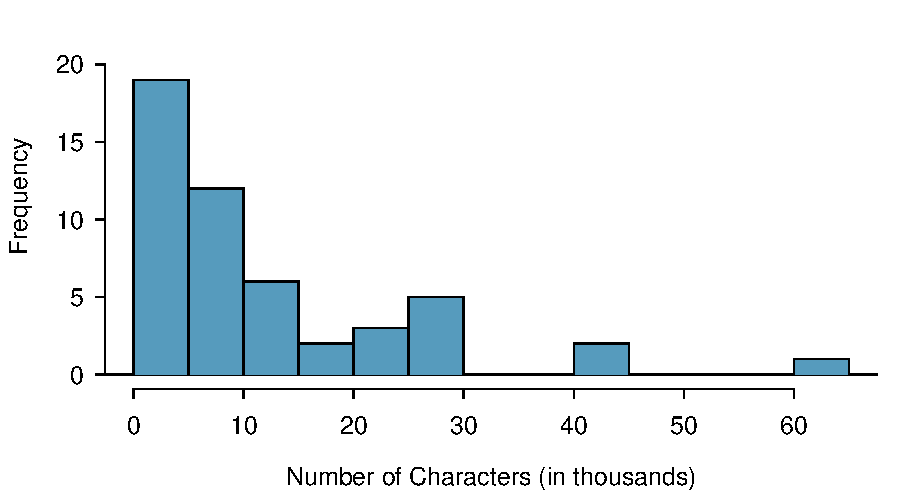
\includegraphics[width=0.75\textwidth]{01/figures/email50NumCharHist/email50NumCharHist} %carsPriceHist/carsPriceHist}
   \caption{Histogram of \var{num\_char}.}
   \label{email50NumCharHist} %carsPriceHist}
\end{figure}

Histograms provide a view of the \term{data density}. Higher bars represent where the data are relatively more common. For instance, there are many more emails with fewer than 15,000 characters than emails with at least 20,000 in the data set. The bars make it especially easy to see how the density of the data changes relative to the number of characters. %: in general, it seems that most emails contain a fairly small number of characters while a small number of emails contain many characters.

Histograms are especially convenient for describing the shape of the data distribution\label{shapeFirstDiscussed}. Figure~\ref{email50NumCharHist} shows that most emails have a relatively small number of characters, while fewer emails have a very large number of characters. When data trail off to the right in this way and have a longer right \hiddenterm{tail}, \index{skew!tail} the shape is said to be \termsub{skewed to the right}{skew!skewed to the right}\footnote{Other ways to describe data skewed to the right: \termsub{right skewed}{skew!right skewed}, \termsub{skewed to the high end}{skew!skewed to the high end}, or \termsub{skewed to the positive end}{skew!skewed to the positive end}.}.

Data sets with the reverse characteristic -- a long, thin tail to the left -- are said to be \termsub{left skewed}{skew!left skewed}. It might also be said that such a distribution has a long left tail. Data sets that show roughly equal trailing off in both directions are called \term{symmetric}. \index{skew!symmetric}

\begin{termBox}{\tBoxTitle{Long tails to identify skew}
When data trail off in one direction, it is called a \term{long tail}. \index{skew!long tail|textbf} If a distribution has a long left tail, it is left skewed. If a distribution has a long right tail, it is right skewed.}
\end{termBox}

\begin{exercise}
Take a look at Figure~\ref{emailCharactersDotPlot} on page~\pageref{emailCharactersDotPlot}. Can you see the skew in the data? Is it easier to see the skew in Figure~\ref{emailCharactersDotPlot} or Figure~\ref{email50NumCharHist}? Comment in the footnote\footnote{While both plots indicate a skewed distribution, it is usually easier to see this characteristic in a histogram. When the data set becomes large, histograms are nearly always employed since the dot plot can become overly crowded with points.}.
\end{exercise}

\begin{exercise}
Besides the mean (since it was labeled), what can you see in Figure~\ref{emailCharactersDotPlot} that you cannot see in \ref{email50NumCharHist}? Answer in the footnote\footnote{Character counts for individual emails.}.
\end{exercise}

In addition to looking at whether a distribution is skewed or symmetric, histograms can be used to identify modes. A \term{mode} is represented by a prominent peak in the distribution\footnote{Another definition of mode, which is not typically used in statistics, is the value with the most occurrences. It is common to have \emph{no} observations with the same values in a data set, which makes this other definition useless for many real data sets.}. There is only one prominent peak in the histogram of \var{num\_char}.

Figure~\ref{singleBiMultiModalPlots} shows histograms that have one, two, and three prominent peaks. Such distributions are called \termsub{unimodal}{modality!unimodal}, \termsub{bimodal}{modality!bimodal}, and \termsub{multimodal}{modality!multimodal}, respectively. Any distribution with more than 2 prominent peaks is called multimodal. Notice that there was one prominent peak in the unimodal distribution with a second less prominent peak that was not counted since it only differs from its neighboring bins by a few observations.
\begin{figure}[h]
   \centering
   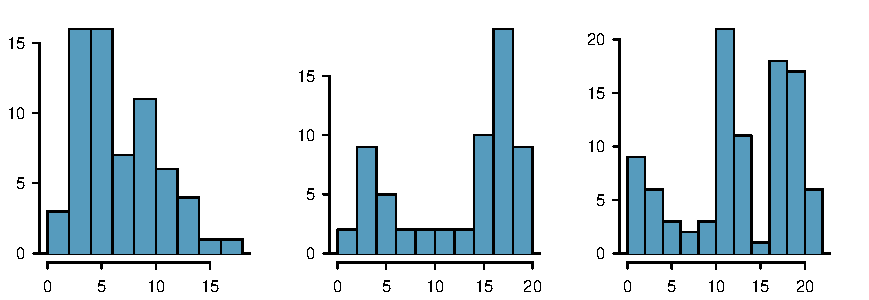
\includegraphics[width=\textwidth]{01/figures/singleBiMultiModalPlots/singleBiMultiModalPlots}
   \caption{Counting only prominent peaks, the distributions are (left to right) unimodal, bimodal, and multimodal.}
   \label{singleBiMultiModalPlots}
\end{figure}

\begin{exercise}
Figure~\ref{email50NumCharHist} reveals only one prominent mode in \var{num\_char}. Is the distribution unimodal, bimodal, or multimodal? Answer in the footnote\footnote{Unimodal. Remember that \emph{uni} stands for 1 like \emph{uni}cycles that have one wheel, and \emph{bi} stands for 2 like \emph{bi}cycles, which have two tires. (We're hoping a \emph{multicycle} will be invented to complete this analogy.)}.
\end{exercise}

\begin{exercise}
Height measurements of young students and adult teachers at a K-3 elementary school were taken. How many modes would you anticipate in this height data set? Answer in the footnote\footnote{There might be two height groups visible in the data set: one of the students and one of the adults. That is, the data are probably bimodal.}.
\end{exercise}

\begin{tipBox}{\tipBoxTitle{Looking for modes}
Looking for modes isn't about finding a clear and correct answer about the number of modes in a distribution, which is why \emph{prominent} is not defined mathematically here. The importance of this examination is to better understand your data and how it might be structured.}
\end{tipBox}

%If you find two or more prominent peaks, the data may arise from two or more subpopulations. Even if the distribution is not bimodal or multimodal, it is certainly not uncommon to reap benefits from grouping data by other variables, which will be discussed casually in Section~\ref{comparingAcrossGroups}.

\subsection{Variance and standard deviation}
\label{variability}

The mean was introduced as a method to describe the center of a data set, but the data's \indexthis{variability}{variability} is also important. Here, we introduce two measures of variability: the variance and the standard deviation. Both of these are very useful in data analysis, even though their formulas are a bit tedious to compute by hand. The standard deviation is the easier of the two to understand, and it roughly describes how far away the typical observation is from the mean.

We call the distance of an observation from its mean its \term{deviation}. Below are the $1^{st}_{}$, $2^{nd}_{}$, and $50^{th}_{}$ deviations for the \var{num\_char} variable:
\begin{align*}
x_1^{}-\bar{x} &= 963 - 12421 = -11459 \hspace{5mm}\text{ } \\
x_2^{}-\bar{x} &= 15586 - 12421 = 3164 \\
			&\ \vdots \\
x_{50}^{}-\bar{x} &= 4371 - 12421 = -8051
\end{align*}
If we square these deviations and then take an average, the result is about equal to the sample \term{variance}\label{varianceIsDefined}, denoted by $s_{}^2$\marginpar[\raggedright$s^2_{}$\\\footnotesize sample variance]{\raggedright$s^2_{}$\\\footnotesize sample variance}:
\begin{eqnarray*}
s_{}^2 &=& \frac{(-11,459)_{}^2 + (3,164)_{}^2 + \cdots + (-8,051)_{}^2}{50-1} \\
	&=& \frac{131,308,681 + 10,010,896 + \cdots + 64,818,601}{49} = 194,172,624
\end{eqnarray*}
(We divide by $n-1$, rather than dividing by $n$, when computing the variance.) Notice that squaring the deviations does two things: (i) it makes large values much larger, seen by comparing $(-11,459)^2$, $(3,164)^2$, and $(-8,051)^2$, and (ii) it gets rid of any negative signs.

The \term{standard deviation} is defined as the square root of the variance:
$$s=\sqrt{194,172,624} = 13,935$$
\marginpar[\raggedright\vspace{-10mm}

$s$\\\footnotesize sample standard deviation]{\raggedright\vspace{-10mm}

$s$\\\footnotesize sample standard deviation}
A subscript of $_x$ may be added to the the variance and standard deviation -- that is, $s_x^2$ and $s_x^{}$ -- as a reminder that these are the variance and standard deviation of the observations represented by $x_1^{}$, $x_2^{}$, ..., $x_n^{}$. These may be omitted when it is clear which data the standard deviation is referencing.

\begin{termBox}{\tBoxTitle{Variance and standard deviation}
The variance is roughly the average squared distance from the mean. The standard deviation is the square root of the variance.}
\end{termBox}

Formulas and methods used to compute the variance and standard deviation for a population are similar to those used for a sample\footnote{The only difference is that the population variance has a division by $n$ instead of $n-1$.}. However, like the mean, the population values have special symbols: $\sigma_{}^2$\marginpar[\raggedright$\sigma_{}^2$\\\footnotesize population variance\\ \hspace{2mm}]{\raggedright$\sigma_{}^2$\\\footnotesize population variance\\ \hspace{2mm}} for the variance and $\sigma$\marginpar[\raggedright$\sigma$\\\footnotesize population standard deviation\\ \hspace{2mm}]{\raggedright$\sigma$\\\footnotesize population standard deviation\\ \hspace{2mm}} for the standard deviation. The symbol $\sigma$ \index{Greek!$\sigma$} is the Greek letter \emph{sigma}\index{Greek!sigma}. As with the sample variance and standard deviation, subscripts such as $_{x}^{}$ can be added to specify which data sets the population variance and standard deviation reference.
\begin{figure}
\centering
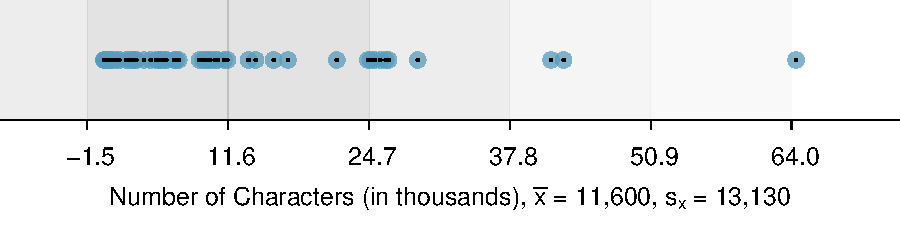
\includegraphics[width=\mycaptionwidth]{01/figures/sdAsRuleForEmailNumChar/sdAsRuleForEmailNumChar} %sdAsRuleForCarsPrice/sdAsRuleForCarsPrice}
\caption{The 70\% within 1 standard deviation and 95\% within 2 is not strict, and it often breaks down for data sets that are extremely skewed. In the \var{num\_char} data, 43 of 50 emails (86\%) are within 1 standard deviation of the mean, 12,422. Additionally, 46 of the 50 emails (92\%) are within 2 standard deviations.}
\label{sdAsRuleForEmailNumChar}
\end{figure}

The standard deviation is useful in considering how close the data are to the mean. Usually about 70\% of the data are within one standard deviation of the mean and 95\% within two standard deviations. However, these percentages can and do vary from one distribution to another. Figure~\ref{severalDiffDistWithSdOf1} shows several different distributions that have the same center and variability but very different shapes.
\begin{figure}
\centering
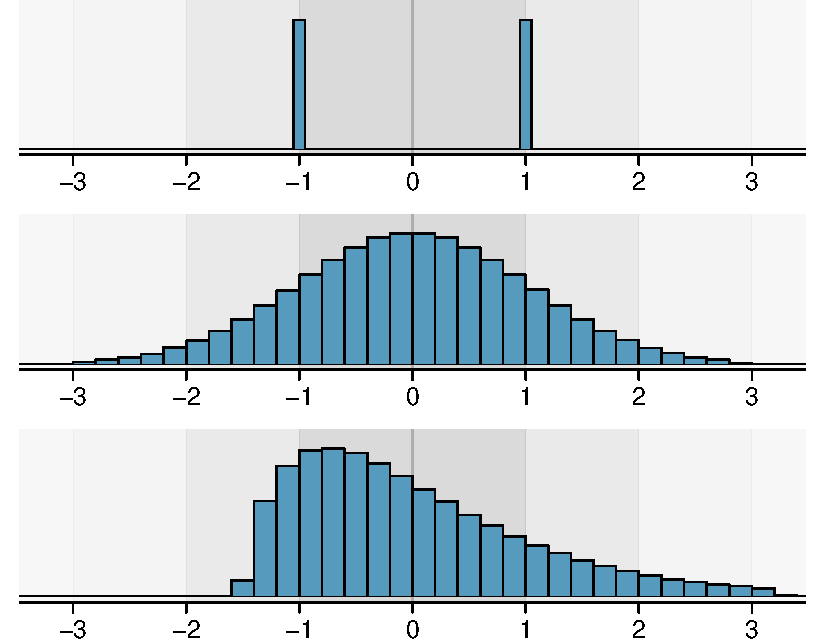
\includegraphics[width=0.7\textwidth]{01/figures/severalDiffDistWithSdOf1/severalDiffDistWithSdOf1}
\caption{Three very different population distributions with the same mean $\mu=0$ and standard deviation $\sigma=1$.\vspace{-3mm}}
\label{severalDiffDistWithSdOf1}
\end{figure}

\begin{exercise}
On page~\pageref{shapeFirstDiscussed}, the concept of shape of a distribution was introduced. A good description of the shape of a distribution should include modality and whether the distribution is symmetric or skewed to one side. Using Figure~\ref{severalDiffDistWithSdOf1} as an example, explain why such a description is important. Answer in the footnote\footnote{Figure~\ref{severalDiffDistWithSdOf1} shows three distributions that look quite different, but all have the same mean, variance, and standard deviation. Using modality, we can distinguish between the first plot (bimodal) and the last two (unimodal). Using skewness, we can distinguish between the last plot (right skewed) and the first two. While a picture, like a histogram, tells a more complete story, we can use modality and shape (symmetry/skew) to characterize basic information about a~distribution.}.
\end{exercise}

\begin{example}{Describe the distribution of the \var{num\_char} variable, shown in Figure~\ref{email50NumCharHist} on page~\pageref{email50NumCharHist}. The description should incorporate the center, variability, and shape of the distribution, and it should also be placed in context: the number of characters in emails. Also note any especially unusual cases.}
The distribution of email character counts is unimodal and very skewed to the high end. Many of the counts fall near the mean at 12,422, and most fall within one standard deviation (13,935) of the mean. There are four very long emails with more than 40,000 characters.
\end{example}

In practice, the variance and standard deviation are sometimes used as a means to an end, where the ``end'' is being able to accurately estimate the uncertainty associated with a sample statistic. For example, in Chapter~\ref{foundationsForInference} we use the variance and standard deviation to assess how close the sample mean is to the population mean.

\begin{tipBox}{\tipBoxTitle{standard deviation describes variability}
Standard deviation is complex mathematically. However, it is not conceptually difficult. It is useful to remember that usually about 70\% of the data are within one standard deviation of the mean and about 95\% are within two standard deviations. However, as seen in Figure~\ref{sdAsRuleForEmailNumChar}, these fractions are not strict rules.}
\end{tipBox}

\subsection{Box plots, quartiles, and the median}

A \term{box plot} summarizes a data set using five statistics while also plotting unusual observations. Figure~\ref{boxPlotLayoutNumVar} provides a vertical dot plot alongside a box plot of the \var{num\_char} variable from the \data{email50} data set.
\begin{figure}[h]
   \centering
   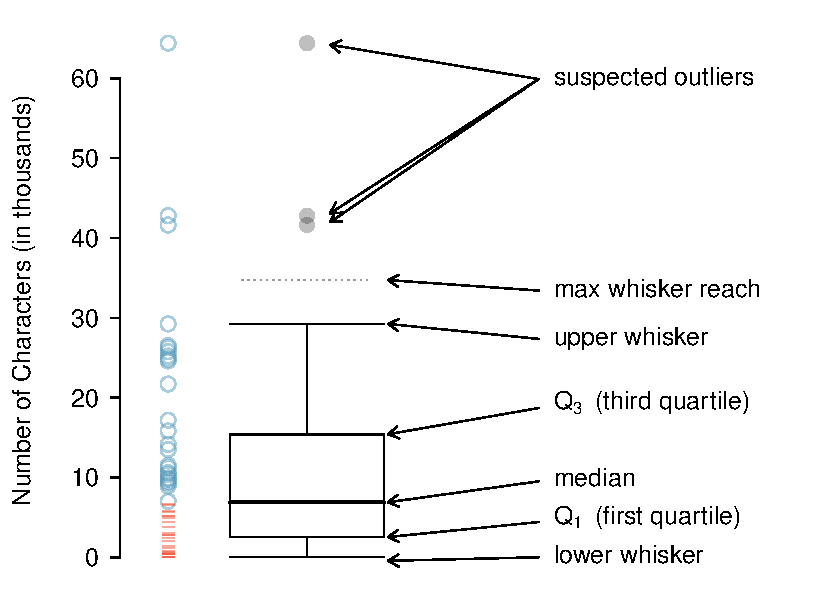
\includegraphics[width=\mycaptionwidth]{01/figures/boxPlotLayoutNumVar/boxPlotLayoutNumVar} %boxPlotLayout/boxPlotLayout}
   \caption{A vertical dot plot next to a labeled box plot of the \var{num\_char} data. The median (6,430.5), splits the data into the bottom 50\% and the top 50\%, marked in the dot plot by horizontal dashes and open circles, respectively.}
   \label{boxPlotLayoutNumVar} %boxPlotLayout}
\end{figure}

The first step in building a box plot is drawing a rectangle to represent the middle 50\% of the data. The total length of the box, shown vertically in Figure~\ref{boxPlotLayoutNumVar}, is called the \term{interquartile range} (\hiddenterm{IQR}, for short). It, like the standard deviation, is a measure of \indexthis{variability}{variability} in data. The more variable the data, the larger the standard deviation and IQR. The two boundaries of the box are called the \term{first quartile} \index{quartile!first quartile} (the $25^{th}$ \hiddenterm{percentile}, i.e. 25\% of the data fall below this value) and the \term{third quartile} \index{quartile!third quartile} (the $75^{th}$ percentile), and these are often labeled $Q_1$ \index{Q$_1$} and $Q_3$\index{Q$_3$}, respectively.

\begin{termBox}{\tBoxTitle{Interquartile range (IQR)}
The \term{interquartile range (IQR)} is the length of the box in a box plot. It is computed as
\begin{eqnarray*}
IQR = Q_3 - Q_1
\end{eqnarray*}
where $Q_1$ and $Q_3$ are the $25^{th}$ and $75^{th}$ percentiles.}
\end{termBox}

The line splitting the box denotes the \term{median}, or the value that splits the data in half. Figure~\ref{boxPlotLayoutNumVar} shows 50\% of the data falling below the median (dashes) and other 50\% falling above the median (hollow circles). There are 50 character counts in the data set (an even number) so the data are perfectly split into two groups of 25. We take the median in this case to be the average of the two observations closest to the $50^{th}$ percentile: $\frac{6,288 + 6,573}{2} = 6,430.5$. When there are an odd number of observations, there will be exactly one observation that splits the data into two halves, and in this case that observation is the median (no average needed).

\begin{termBox}{\tBoxTitle{Median: the number in the middle}
If the data are ordered from smallest to largest, the \term{median} is the observation right in the middle. If there are an even number of observations, there will be two values in the middle, and the median is taken as their average.}
\end{termBox}

\begin{exercise}
What percent of the data fall between $Q_1$ and the median? How much between the median and $Q_3$? Answers in the footnote\footnote{Since $Q_1$ and $Q_3$ capture the middle 50\% of the data and the median splits the data in the middle, 25\% of the data fall between $Q_1$ and the median, and another 25\% falls between the median and $Q_3$.}.
\end{exercise}

Extending out from the box, the \term{whiskers} attempt to capture the data outside of the box, however, their reach is never allowed to be more than $1.5*IQR$.\footnote{While the choice of exactly 1.5 is arbitrary, it is the most commonly used value for box plots.} They grab everything within this reach. In Figure~\ref{boxPlotLayoutNumVar}, the upper whisker cannot extend to the last four points, which is beyond $Q_3 + 1.5*IQR$, and so it extends only to the last point below this limit. The lower whisker stops at the lowest value, 53, since there is no additional data to reach; the lower whisker limit is not shown in the figure because the plot does not extend down to $Q_1 - 1.5*IQR$. In a sense, the box is like the body of the box plot and the whiskers are like its arms trying to reach the rest of the data.

Any observation that lies beyond the whiskers is labeled with a dot. The purpose of labeling these points -- instead of just extending the whiskers to the minimum and maximum observed values -- is to help identify any observations that appear to be unusually distant from the rest of the data. Unusually distant observations are called \termsub{outliers}{outlier}. In the case of the \var{num\_char} variable, the emails with character counts of 43,656, 44,899, 48,442, and 56,529 are potential outliers.

\begin{termBox}{\tBoxTitle{Outliers are extreme}
An \term{outlier} is an observation that appears extreme relative to the rest of the data.}
\end{termBox}


\begin{tipBox}{\tipBoxTitle{Why it is important to look for outliers}
Examination of data for possible outliers serves many useful purposes, including\vspace{-2mm}
\begin{enumerate}
\setlength{\itemsep}{0mm}
\item Identifying \indexthis{extreme skew}{skew!extreme skew} in the distribution.
%\item Inferring that seemingly unusual cases are actually commonplace for a variable.
\item Identifying data collection or entry errors. For instance, we re-examined the email purported to have 56,529 characters to ensure this value was accurate.
\item Providing insights into interesting phenomena with the data.
\end{enumerate}}
%The identification of outliers is not actually what is important, which is why no rigid definition for outlier is provided. What is important is to examine and take special note of \emph{suspected} outliers and why they are extreme compared to the rest of the data.}
\end{tipBox}

\begin{exercise}
The observation 56,529, a suspected outlier, was found to be an accurate observation. What would such an observation suggest about the nature of character counts in emails? Answer in the footnote\footnote{That occasionally there may be extremely long emails.}. % (In Section~\ref{}, we will see that those emails with the most characters actually contain much styling in the form of HTML, which contributes to the large number of characters.)}.
\end{exercise}

\begin{exercise}
Using Figure~\ref{boxPlotLayoutNumVar}, estimate the following values for \var{num\_char} in the \data{email50} data set: (a) $Q_1$, (b) $Q_3$, and (c) IQR. Estimates are provided in the footnote\footnote{Rough guesses: $Q_1=2,000$, $Q_3=18,000$, $\text{IQR}=Q_3 - Q_1 = 16,000$. (The true values: $Q_1=1,894$, $Q_3=18,184$, $\text{IQR} = 16,290$.)}.
\end{exercise}

\subsection{Robust statistics}

How are the \indexthis{sample statistics}{sample statistic} of the \data{num\_char} data set affected by the outlier observation, 56,529? What would have happened if this email wasn't observed? What would happen to these \indexthis{summary statistics}{summary statistic} if the outlier at 56,529 had been even larger, say 200,000? These scenarios are plotted alongside the original data in Figure~\ref{email50NumCharDotPlotRobustEx}, and sample statistics are computed under each scenario in Table~\ref{robustOrNotTable}.
\begin{figure}[ht]
\centering
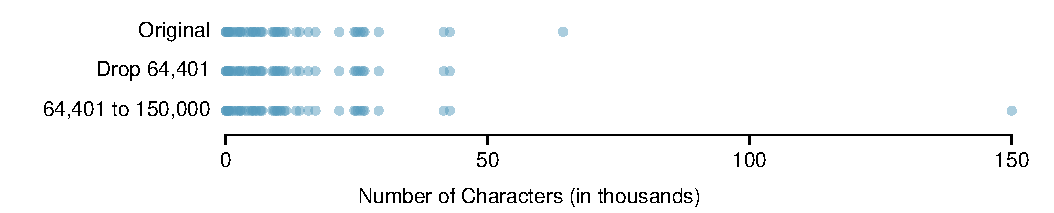
\includegraphics[width=\textwidth]{01/figures/email50NumCharDotPlotRobustEx/email50NumCharDotPlotRobustEx} %carsPriceDotPlotRobustEx/carsPriceDotPlotRobustEx}
\caption{Dot plots of the original character count data and two modified data sets.}
\label{email50NumCharDotPlotRobustEx}
\end{figure}
\begin{table}[ht]
\centering
\begin{tabular}{l c cc c cc}
  \hline
& \hspace{0mm} & \multicolumn{2}{c}{\bf robust} & \hspace{2mm} & \multicolumn{2}{c}{\bf not robust} \\
scenario && median & IQR && $\bar{x}$ & $s$ \\ 
  \hline
original \var{num\_char} data 	&& 6,430.5 & 16,290 && 12,422 & 13,935 \\
% library(openintro); data(email50); d <- email50$num_char; median(d); IQR(d); mean(d); sd(d)
drop 56,529 observation		&& 6,288 & 15,835 && 11,522 & 12,524 \\
% library(openintro); data(email50); d <- email50$num_char; d <- d[-which.max(d)]; median(d); IQR(d); mean(d); sd(d)
move 56,529 to 100,000		&& 6430.5 & 16,290 && 13,291 & 17,613 \\
% library(openintro); data(email50); d <- email50$num_char; d[which.max(d)] <- 100000; median(d); IQR(d); mean(d); sd(d)
%original \var{price} data && 17.25 & 15.30 && 19.99 & 11.51 \\ 
%move \$61,900 to \$200,000 && 17.25 & 15.30 && 22.55 & 26.53 \\ 
%move \$7,400 to \$200,000 && 18.30 & 15.45 && 26.12 & 35.79 \\ 
   \hline
\end{tabular}
\caption{A comparison of how the median, IQR, mean ($\bar{x}$), and standard deviation ($s$) change when extreme observations are in play.}
\label{robustOrNotTable}
\end{table}

\begin{exercise}
(a) Which is more affected by extreme observations, the mean or median? Table~\ref{robustOrNotTable} may be helpful. (b) Is the standard deviation or IQR more affected by extreme observations? Brief answers in the footnote\footnote{(a) Mean is affected more. (b) Standard deviation is affected more.}.
\end{exercise}

The median and IQR are called \term{robust estimates} because extreme observations have little effect on their values. The mean and standard deviation are much more affected by changes in extreme observations.

\begin{exercise}
Examine Table~\ref{robustOrNotTable}. Why doesn't the median or IQR change much from one scenario to the next? Answer in the footnote\footnote{These values are largely defined by values near $Q_1$, the median, and $Q_3$. Since values in these regions are largely stable -- there aren't large jumps between observations -- the median and IQR estimates are relatively stable.}.
\end{exercise}

\begin{exercise}
The distribution of vehicle prices tends to be right-skewed, with a few luxury and sports cars lingering out far into the right tail. If you were searching for a new car and cared about price, should you be more interested in the mean price of vehicle's sold or the median vehicle price if you were in the market for a regular car? Answer in the footnote\footnote{Buyers of a ``regular car'' should be concerned about the median price. High-end car sales can drastically inflate the mean price while the median will be more robust to the influence of those sales.}.
\end{exercise}

\subsection{Transforming data (special topic)}

When data are extremely skewed, we sometimes transform them so they are easier to model.
%\begin{example}{Consider the distribution of \var{num\_char}, shown in Figures~\ref{email50NumCharHist} and~\ref{boxPlotLayoutNumVar} to be an extremely skewed distribution.}
%\end{example}
%We see that there are many values near zero and then data trails off to the right. It might be more natural to look at the distribution of these data after they've been transformed.
Consider the histogram of salaries for Major League Baseball players' salaries from 2010, which is shown in Figure~\ref{histMLBSalariesReg}.
\begin{figure}[ht]
\centering
\subfigure[]{
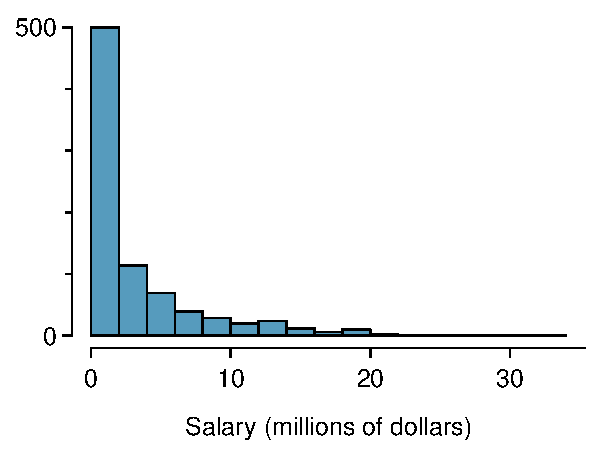
\includegraphics[width=0.46\textwidth]{01/figures/histMLBSalaries/histMLBSalariesReg}
\label{histMLBSalariesReg}
}
\subfigure[]{
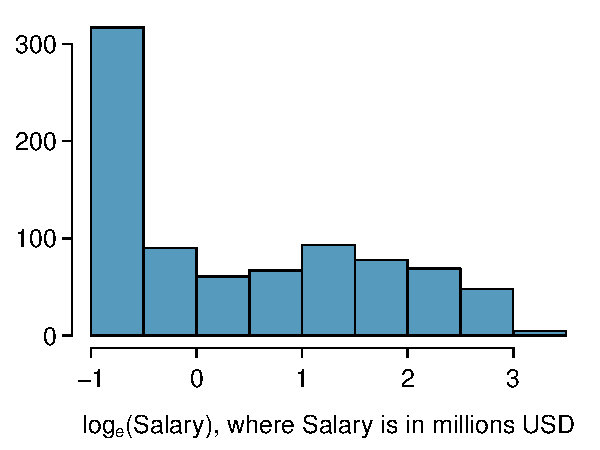
\includegraphics[width=0.46\textwidth]{01/figures/histMLBSalaries/histMLBSalariesLog}
\label{histMLBSalariesLog}
}
\caption{\subref{histMLBSalariesReg} Histogram of MLB player salaries for 2010, in millions of dollars. \subref{histMLBSalariesLog} Histogram of the log-transformed MLB player salaries for 2010.}
\label{histMLBSalaries}
\end{figure}

\begin{example}{The histogram of MLB player salaries is useful in that we can see the data are highly skewed and centered (as gauged by the median) at about \$1 million. What isn't useful about this plot?}
Most of the data are collected into one bin in the histogram and the data are so strongly skewed that some details in the data are obscured.
\end{example}

There are some standard transformations that are often applied when much of the data cluster near zero (relative to the larger values in the data set) and all observations are positive. A \term{transformation} is a rescaling of the data using a function. For instance, a plot of the natural logarithm\footnote{Statisticians often write the natural logarithm as $\log$. You might be more familiar with it being written as $\ln$.} of player salaries results in a new histogram in Figure~\ref{histMLBSalariesLog}. Transformed data are sometimes easier to work with when applying statistical models because the transformed data are much less skewed and outliers are usually less extreme. %The extreme skew in the pre-transformed data was so strong that it would add an extra layer of modeling complexity.

%\begin{exercise}
%What do you notice in Figure~\ref{histMLBSalariesReg} that you were unable to see in Figure~\ref{histMLBSalariesLog}?
%\end{exercise}

Transformations can also be applied to one or both variables in a scatterplot. A scatterplot of the \var{lines} and \var{num\_char} variables is shown in Figure~\ref{email50LinesCharactersMod}, which was earlier shown in Figure~\ref{email50LinesCharacters}. %scatterMammalGestLSReg} representing mammal lifespans against the time of gestation (time spent in the womb).
We can see a positive association between the variables and that many observations are clustered near zero.
%There seems to be a positive association between these two variables.
In Chapter~\ref{linRegrForTwoVar}, we might want to use a straight line to model the data. However, we'll find that the data in their current state cannot be modeled very well. Figure~\ref{email50LinesCharactersModLog} shows a scatterplot where both the \var{lines} and \var{num\_char} variables have been transformed using a log (base $e$) transformation. While there is a positive association in each plot, the transformed data show a steadier trend, which is easier to model than the untransformed data.
\begin{figure}
\centering
\subfigure[]{
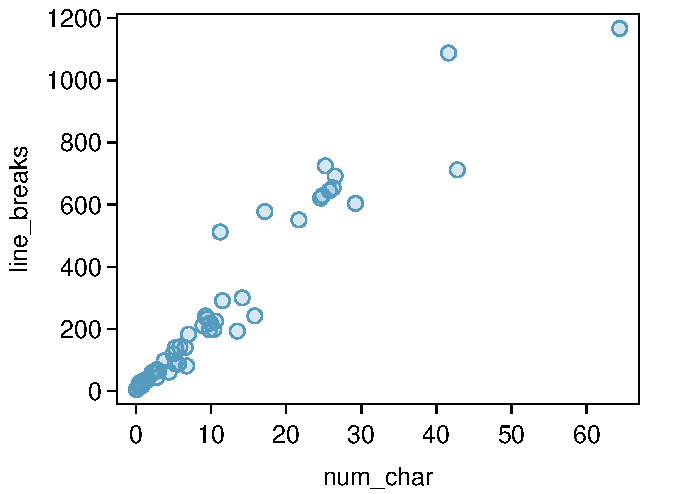
\includegraphics[width=0.46\textwidth]{01/figures/email50LinesCharactersMod/email50LinesCharactersMod}
\label{email50LinesCharactersMod}
%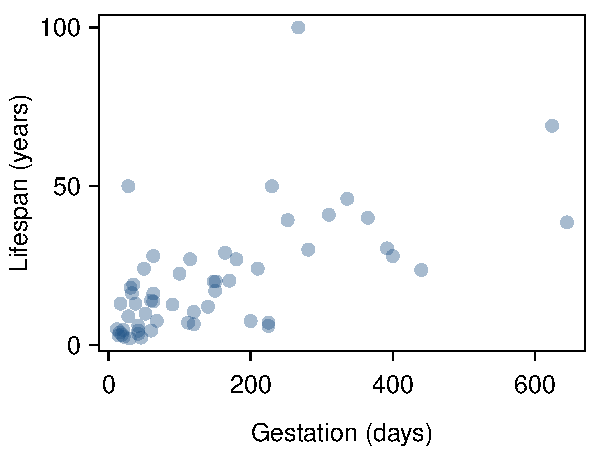
\includegraphics[width=0.46\textwidth]{01/figures/scatterMammalGestLS/scatterMammalGestLSReg}
%\label{scatterMammalGestLSReg}
}
\subfigure[]{
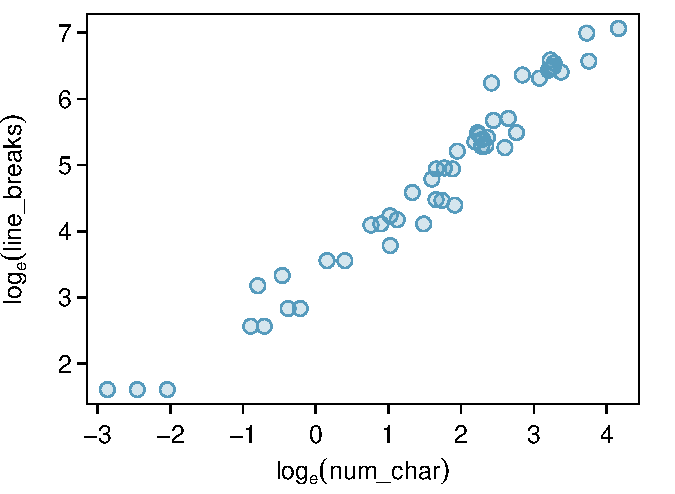
\includegraphics[width=0.46\textwidth]{01/figures/email50LinesCharactersMod/email50LinesCharactersModLog} %scatterMammalGestLS/scatterMammalGestLSTra}
\label{email50LinesCharactersModLog} %scatterMammalGestLSTra}
}
\caption{\subref{email50LinesCharactersMod} Scatterplot of \var{lines} against \var{num\_char} for 50 emails. \subref{email50LinesCharactersModLog} A scatterplot of the same data but where each variable has been log-transformed.}
\label{email50LinesCharactersModMain} %scatterMammalGestLS}
\end{figure}

Other transformations other than the logarithm can be useful, too. For instance, the square root ($\sqrt{\text{original observation}}$) and inverse ($\frac{1}{\text{original observation}}$) are regularly used by statisticians. Common goals in transforming data are to see the data structure differently, reduce skew, assist in modeling, or straighten a nonlinear relationship in a scatterplot.

\index{data!email50|)}

%\begin{example}{Examine both plots in Figure~\ref{email50LinesCharactersModMain}. Here we see that both variables are much more uniform over the range of values after transformation. What does this suggest about an analysis that considers just one of these variables?}
%It may be useful to characterize the 
%\end{example}

\subsection{Mapping data (special topic)}

\index{data!county|(}
\index{intensity map|(}

The \data{county} data set offers many numerical variables that we could plot using dot plots, scatterplots, or box plots, but these miss the true nature of the data. Rather, when we encounter geographic data, we should map it using an \term{intensity map}, where colors are used to show higher and lower values of a variable. Figures~\ref{countyIntensityMaps1} and~\ref{countyIntensityMaps2} shows intensity maps for the \var{fed\_spend}, \var{poverty}, \var{homeownership}, and \var{med\_income} variables. The color key indicates which colors correspond to which values. Note that the intensity maps are not generally very helpful for getting precise values in any given county, but they are very helpful for seeing geographic trends and generating interesting research questions.

\begin{figure}
\centering
\subfigure[]{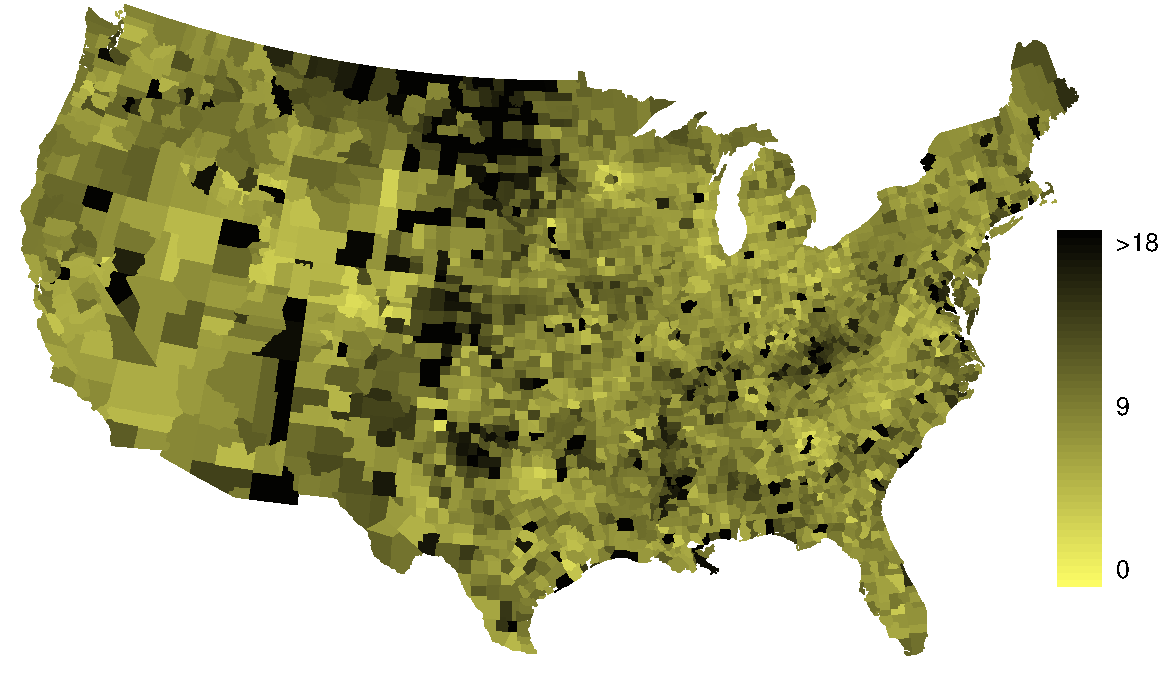
\includegraphics[width=\textwidth]{01/figures/countyIntensityMaps/countyFedSpendMap}\label{countyFedSpendMap}}
\subfigure[]{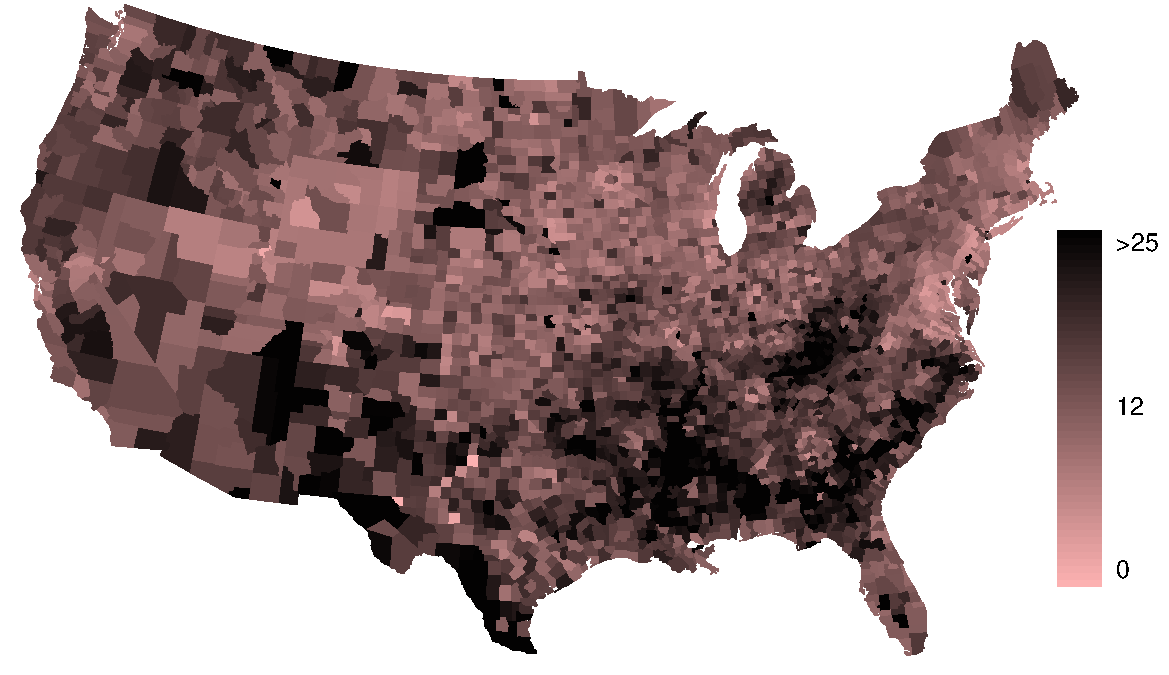
\includegraphics[width=\textwidth]{01/figures/countyIntensityMaps/countyPovertyMap}\label{countyPovertyMap}}
\caption{\subref{countyFedSpendMap} Map of federal spending (dollars per capita). \subref{countyPovertyMap} Intensity map of poverty rate (percent).}
\label{countyIntensityMaps1}
\end{figure}
\begin{figure}
\centering
\subfigure[]{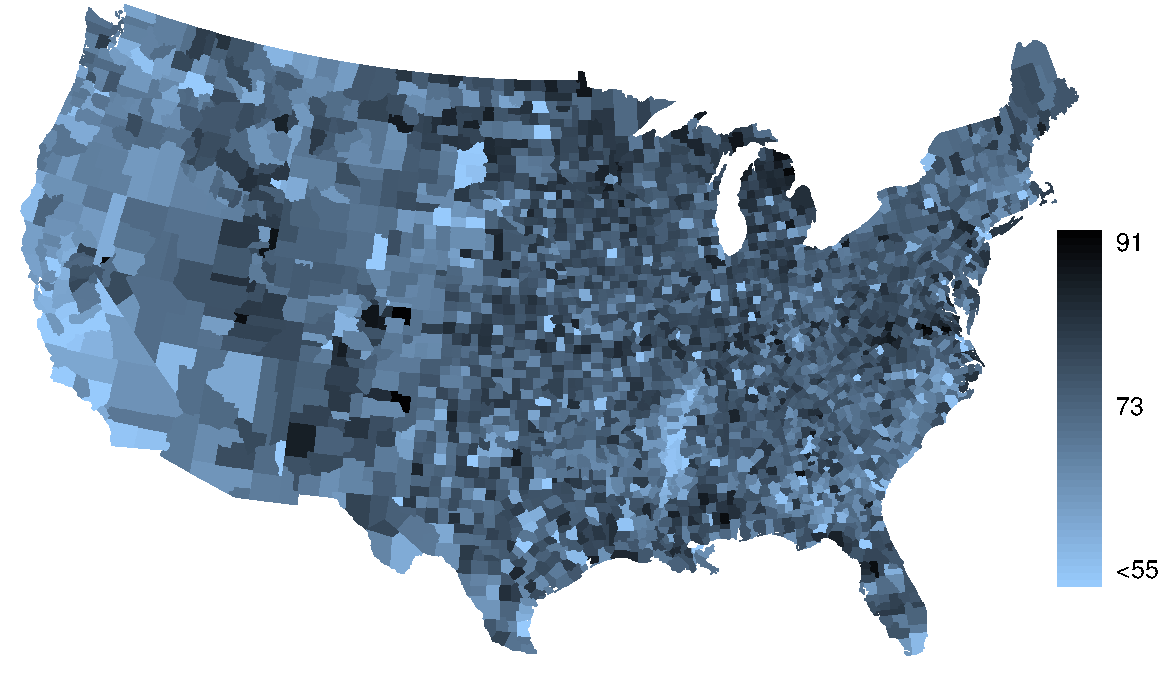
\includegraphics[width=\textwidth]{01/figures/countyIntensityMaps/countyHomeownershipMap}\label{countyHomeownershipMap}}
\subfigure[]{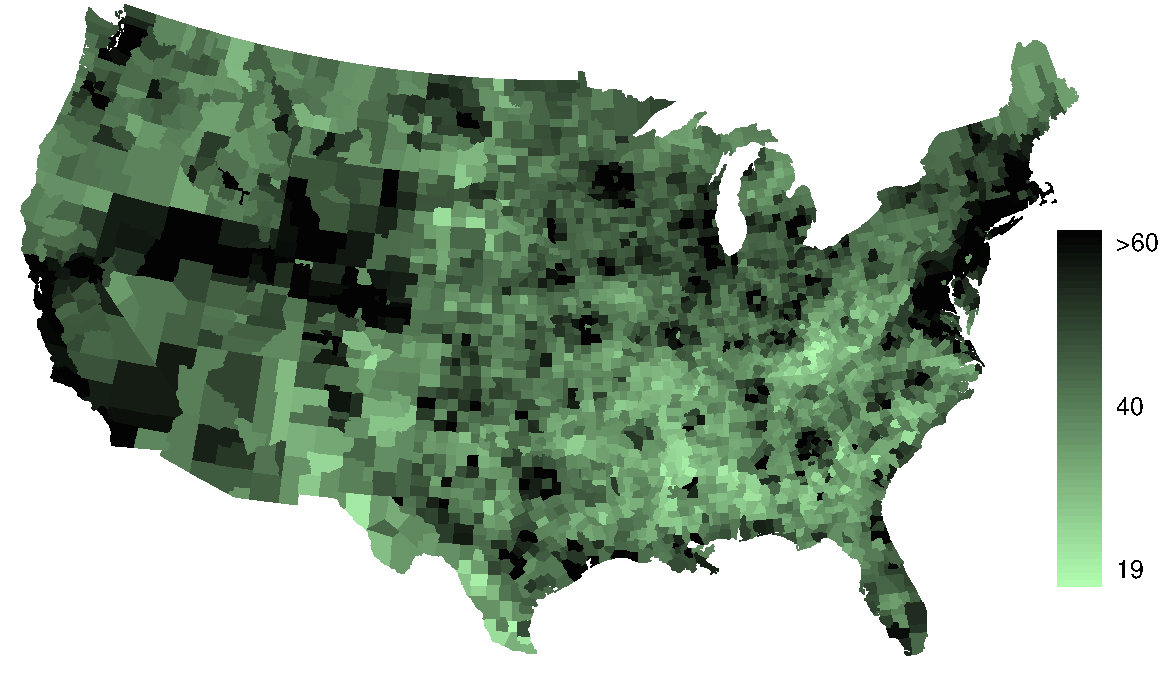
\includegraphics[width=\textwidth]{01/figures/countyIntensityMaps/countyMedIncomeMap}\label{countyMedIncomeMap}}
\caption{\subref{countyHomeownershipMap} Intensity map of homeownership rate (percent). \subref{countyMedIncomeMap} Intensity map of median household income (\$1000s).}
\label{countyIntensityMaps2}
\end{figure}

\begin{example}{What interesting features are evident in the \var{fed\_spend} and \var{poverty} intensity maps?}
The federal spending intensity map shows substantial spending in the Dakotas and along the central-to-western part of the Canadian border. We wonder if this federal spending may be in some way related to the oil boom in this area of the country. There are also several other patches of federal spending that we might identify, such as a vertical strip in eastern Utah and Arizona and the area where Colorado, Nebraska, and Kansas meet. It is also worth noting that there are seemingly random counties that have very high federal spending relative to their neighbors. If we looked into these data further and did not cap the federal spending range at \$18 per capita, we would actually find that some counties have extremely high federal spending while there is almost no federal spending in the neighboring counties. This phenomenon would be interesting to investigate and may correspond to government facilities that house many employees, military bases, or large contracts with companies.

Poverty rates are evidently higher in a few locations. Notably, the deep south shows higher poverty rates, as does the southwest border of Texas. The vertical strip of eastern Utah and Arizona, noted above for its higher federal spending, also appears to have higher rates of poverty (though generally little correspondence is seen between the two variables).  High poverty rates are evident in the Mississippi flood plains a little north of New Orleans and also in a large section of Kentucky and West Virginia.
\end{example}

\begin{exercise}
What interesting features are evident in the \var{med\_income} intensity map? Answer in the footnote\footnote{Note: answers will vary. There is a very strong correspondence between high earning and metropolitan areas. You might look for large cities you are familiar with and try to spot them on the map as dark spots.}.
\end{exercise}

\index{intensity map|)}
\index{data!county|)}


\section{Considering categorical data}
\label{categoricalData}

\index{data!email|(}

Like numerical data, categorical data can also be organized and analyzed. In this section, tables and other basic tools for categorical data are introduced that will be used throughout this book. The \data{email50} data set represents a sample from a larger email data set called \data{email}. This larger data set contains information on 2,435 emails and all the same variables. In this section, we will examine whether the presence of numbers, small or large, provide any useful value in classifying email as spam or not spam.

%In this section we investigate three variables: \var{html}, \var{
%whether a message was written as text or HTML (emails with bolding, tables, or images are usually in HTML), whether an exclamation point is in the email subject and whether the email contains HTML encoding -- have an association with an email being spam.

\subsection{Contingency tables and bar plots}

\Comment{Note: bar plots were moved from the next subsection to this subsection.}

Table~\ref{emailSpamNumberTableTotals} summarizes two variables: \var{spam} and \var{number}. Recall that \var{number} is a categorical variables describes whether an email contains no numbers, only small numbers (values under 1 million), or at least one big number (a value of 1 million or more). A table that summarizes data for two categorical variables in this way is called a \term{contingency table}. Each number in the table represents the number of times a particular combination of variable outcomes occurred. For example, the number 39 corresponds to the number of emails in the data set that are spam \emph{and} had no number listed in the email. Row and column totals are also included. The \term{row totals} \index{contingency table!row totals} equal the total counts across each row (e.g. $39 + 48 + 17 = 104$), and \term{column totals} \index{contingency table!column totals} are total counts down each column.

A table for a single variable is called a \term{frequency table}. Table~\ref{emailNumberTable} is a frequency table for the \var{number} variable. If we replaced the counts with percentages or proportions, the table would be called a \term{relative frequency table}.

\begin{table}[ht]
\centering
\begin{tabular}{ll  ccc  rr}
& & \multicolumn{3}{c}{\bf \var{number}} & \\
  \cline{3-5}
& & none & small & big & total & \hspace{2mm}\  \\ 
  \cline{2-6}
						 & spam &  39 & 48 & 17 & 104 \\ 
\raisebox{1.5ex}[0pt]{\var{spam}} & not spam &  293 & 1951 & 87 & 2331 \\ 
  \cline{2-6}
& total & 332 & 1999 & 104 & 2435 \\
  \cline{2-6}
\end{tabular}
\caption{A contingency table for \var{spam} and \var{number}.}
\label{emailSpamNumberTableTotals}
%library(openintro); library(xtable); data(email); xtable(table(email[,c("spam", "number")]))
\end{table}

\begin{table}[htb]
\centering
\begin{tabular}{cccc}
  \hline
none & small & big & total \\ 
 % \grayline
 332 & 1999 & 104 & 2435 \\
   \hline
\end{tabular}
\caption{A frequency table for the \var{number} variable.}
\label{emailNumberTable}
\end{table}
%library(openintro); library(xtable); data(email); xtable(table(email[,c("html")]))

\begin{exercise}
Why is Table~\ref{emailNumberTable} redundant if Table~\ref{emailSpamNumberTableTotals} is provided? Answer in the footnote\footnote{The column totals shown in Table~\ref{emailSpamNumberTableTotals} represent the frequency table exactly.}.
\end{exercise}

%To make the rest of this section a little more interesting, we are going to generate an expanded contingency table that incorporates \var{spam}, \var{html}, and \var{big\_number}, shown in Table~\ref{emailSpamHTMLBigNumberTableTotals}. We will have the two levels of \var{spam} represented in the contingency table rows and the combinations of the other variables represented as columns.

%\begin{table}[ht]
%\centering
%\begin{tabular}{l | cccc | r}
%  \hline
% & text		    & html		    & text		     & html		  &  \\ 
% & no big number & no big number & big number & big number & total \\ 
%  \hline
%spam &  22 &   4 &  20 &   3 & 49 \\ 
%not spam &  182 &   7 & 556 &  31 & 776 \\ 
%   \hline
%total & 204 & 11 & 576 & 34 & 825 \\
%   \hline
%\end{tabular}
%\caption{A contingency table for \var{spam} against the combinations of \var{html} and \var{big\_number}.}
%\label{emailSpamHTMLBigNumberTableTotals}
%%library(openintro); library(xtable); data(email); y <- paste(email$html, email$big_number); xtable(table(data.frame(email$spam, y)))
%\end{table}

A bar plot is a common way to display a single categorical variable. The left panel of Figure~\ref{emailNumberBarPlot} shows a \term{bar plot} for the \var{number} variable. In the right panel, the counts were converted into proportions (e.g. $332/2435=0.136$ for \resp{none}), 
%making it easy to compare how about often different outcomes occur irrespective of sample size.
showing the fraction of the whole that are in each category.
\begin{figure}[bht]
   \centering
   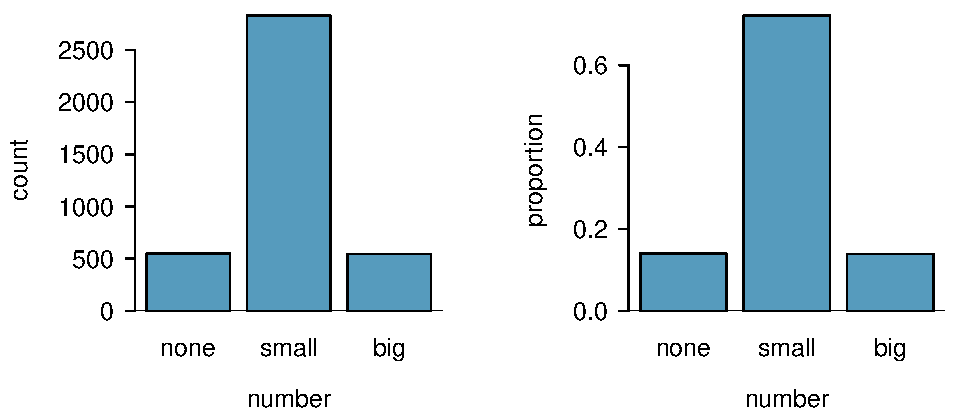
\includegraphics[height=2.3in]{01/figures/emailNumberBarPlot/emailNumberBarPlot}
   \caption{Two bar plots of \var{number}. The left panel shows the counts and the right panel the proportions in each group.}
   \label{emailNumberBarPlot} %typeBarPlot}
\end{figure}


\subsection{Row and column proportions}

%\begin{exercise}
%Which of the following statements would be more useful to an auto executive? (1) 21 cars in our sample were small vehicles. (2) 38.9\% of the cars in our sample were small vehicles. Comment in the footnote\footnote{Even if the sample size (54) was provided in the first statement, the auto exec would probably just be trying to figure out the proportion in her head.}.
%\end{exercise}

%\begin{tipBox}{\tipBoxTitle{data set notation}
%Sometimes the values \resp{1} and \resp{0} are used as the outcomes for a categorical variable if it only has two levels. For instance, if there were only \resp{small} and \resp{large} cars, we could have used \resp{1} to represent \resp{small} and \resp{0} to represent \resp{large} in the \var{type} variable.}
%\end{tipBox}

Table~\ref{rowPropSpamNumber} shows the row proportions for Table~\ref{emailSpamNumberTableTotals}. The \termsub{row proportions}{contingency table!row proportions} are computed as the counts divided by their row totals. The count 39 at the intersection of \resp{spam} and \resp{none} is replaced by $39/104=0.375$, i.e. 39 divided by its row total, 104. So what does 0.375 represent? It corresponds to the proportion of spam emails in the sample that do not have any numbers.
\begin{table}[ht]
\centering
\begin{tabular}{l rrr r}
  \hline
 & none & small & big & total \\ 
  \hline
spam &  $39/104 = 0.375$ & $48/104 = 0.462$ & $17/104 = 0.163$ & 1.000 \\ 
not spam &  $293/2331 = 0.126$ & $1951/2331 = 0.837$ & $87/2331 = 0.037$ & 1.000 \\ 
   \hline
total & $332/2435 = 0.136$ & $1999/2435 = 0.821$ & $104/2435 = 0.043$ & 1.000 \\
  \hline
\end{tabular}
\caption{A contingency table with row proportions for the \var{spam} and \var{number} variables.}
\label{rowPropSpamNumber}
% library(openintro); data(email); g <- table(email$spam, email$number)[2:1,]; g / rep(rowSums(g), 3)
\end{table}

A contingency table of the column proportions is computed in a similar way, where each \termsub{column proportion}{contingency table!column proportion} is computed as the count divided by the corresponding column total. Table~\ref{colPropSpamNumber} shows such a table, and here the value 0.117 represents the proportion of emails with no numbers that are spam. If we look across the rows in this table, we also can note that the proportions are not constant. This is important: it means that the amount of spam varies across the levels of \var{number} and that the two variables are associated (i.e. there is an apparent relationship). We could have made a similar comparison in Table~\ref{rowPropSpamNumber} to check for independence (i.e. the lack of an association), though we would have looked down the columns in that case to see if the fraction of emails with no numbers, small numbers, and big numbers varied from \resp{spam} to \resp{not~spam}.
\begin{table}[ht]
\centering\small
\begin{tabular}{l rrr r}
  \hline
 & none & small & big & total \\ 
  \hline
spam &  $39/332 = 0.117$ & $48/1999 = 0.024$ & $17/104 = 0.163$ & $104/2435 = 0.043$ \\ 
not spam &  $293/332 = 0.883$ & $1951/1999 = 0.976$ & $87/104 = 0.837$ & $2331/2435 = 0.957$ \\ 
   \hline
total & 1.000 & 1.000 & 1.000 & 1.000 \\
   \hline
\end{tabular}
\caption{A contingency table with column proportions for the \var{spam} and \var{number} variables.}
\label{colPropSpamNumber}
% library(openintro); data(email); g <- table(email$spam, email$number)[2:1,]; g / rep(colSums(g), rep(2, 3))
\end{table}

\begin{exercise}
What does 0.462 represent in Table~\ref{rowPropSpamNumber}? What does 0.024 represent in Table~\ref{colPropSpamNumber}? Answers in the footnote\footnote{0.462 represents the proportion of spam emails that had a small number. 0.024 represents the fraction of emails with small numbers that are spam.}.
\end{exercise}

\begin{exercise}
What does 0.037 represent in Table~\ref{rowPropSpamNumber}? What does 0.837 represent in the Table~\ref{colPropSpamNumber}? Answers in the footnote\footnote{0.037 represents the fraction of non-spam email that had a big number. 0.837 represents the fraction of emails with big numbers that are non-spam emails.}.
\end{exercise}

\begin{example}{Software engineers use statistics to filter spam from incoming email messages. By noting specific characteristics of an email, an engineer may be able to classify some emails as spam or not spam with high accuracy. One of those characteristics is whether the email contains no numbers, small numbers, or big numbers. Another characteristic is whether or not an email has any HTML content. A contingency table for the \var{spam} and \var{html} variables from the \data{email} data set are shown in Table~\ref{emailSpamHTMLTableTotals}. Which would be more helpful to a statistician hoping to classify email as spam or regular email: row or column proportions?} \label{weighingRowColumnProportions}
The interest lies in how the \var{spam} changes based on \var{html}. This corresponds to the column proportions: the proportion of spam in plain text emails and the proportion of emails in HTML emails.

We can see that a higher fraction of plain text emails are spam than compared to HTML emails. However, it is worth noting that this information alone is insufficient to classify an email as spam or not spam, as a vast majority of plain text emails are not spam. Yet, when we carefully combine this information with many other characteristics, a topic of Chapter~\ref{multipleRegressionAndANOVA}, we stand a reasonable chance of being able to classify some email as spam or not spam. %Appethods for classifying email as spam or not spam is a subject of Chapter~\ref{}.
\end{example}

%\begin{exercise}
%Table~\ref{possumPopSexContTable} is a contingency table for the \data{possum} data set for the \var{pop} (living location) and \var{sex} variables. Which variable makes more sense as an explanatory variable? Answer in the footnote\footnote{It makes more sense for living location to affect the proportion of males to females in the population. The reverse cannot be entirely ruled out: it might be that possums migrate based on gender, although this seems less likely.}.
%\end{exercise}

%\begin{exercise} \label{weighingRowColumnProportions}
%If \var{pop} (living location) is the explanatory variable and \var{sex} the response, which do you think would be more interesting: row or column proportions? Answer in the footnote\footnote{The interest lies in how the response changes based on the explanatory variable. This corresponds to the row proportions here: the proportion of males/females in each location.% The column proportions correspond to what proportion of the sampled females and males are in each region. (If you need convincing that these are the actual meanings of the row and column proportions in these cases, construct each row and column proportion table.% You can do so in R by using the commands \rcom{prop.table(table(possum[,c('pop', 'sex')]), 1)} and \rcom{prop.table(table(possum[,c('pop', 'sex')]), 2)} after loading the data in R -- see Section~\ref{introductoryMethodsInR}.
%)}.
%\end{exercise}
\begin{table}[ht]
\centering
\begin{tabular}{l cc r}
  \hline
 & text & HTML & total \\ 
  \hline
spam & 58 & 46  & 104 \\ 
not spam & 603 & 1728  & 2331 \\ 
   \hline
total & 661 & 1774 & 2435 \\
   \hline
\end{tabular}
\caption{A contingency table for \var{spam} and \var{html}.}
\label{emailSpamHTMLTableTotals}
%library(openintro); library(xtable); data(email); xtable(table(email[,c("spam", "html")]))
\end{table}

Example~\ref{weighingRowColumnProportions} points out that row and column proportions are not created equal. It is important to consider each before settling on one to ensure that the most useful table is constructed.

\begin{exercise}
Look back to Tables~\ref{rowPropSpamNumber} and~\ref{colPropSpamNumber}. Which would be more useful to someone hoping to identify spam emails using the \var{number} variable? Answer in the footnote\footnote{Table~\ref{colPropSpamNumber} will probably be most useful. From that table, we can see that emails with small numbers are very rarely spam while about 11.7\% of emails with no numbers are spam and 16.3\% of emails with big numbers are spam.}. % In general, a spam filter never knows with certainty whether an email is spam or not, it just makes a very well-informed guess.}.
\end{exercise}

%In Chapter~\ref{multipleRegressionAndANOVA}, we will learn methods for classifying spam that consider several email characteristics simultaneously.

\subsection{Segmented bar and mosaic plots}
\label{segmentedBarPlotsAndIndependence}

Contingency tables using row or column proportions are especially useful for examining how two categorical variables are related. Segmented bar and mosaic plots provide a way to put these tables into a graphical form.

A \termsub{segmented bar plot}{bar plot!segmented bar plot} is a graphical display of contingency table information. For example, a segmented bar plot representing Table~\ref{emailSpamNumberTableTotals} is shown in Figure~\ref{emailSpamNumberSegBar}, where we have first created a bar plot using the \var{number} variable and then broken down each group by the levels of \var{spam}. The row proportions of Table~\ref{colPropSpamNumber} have been translated into a standardized segmented bar plot in Figure~\ref{emailSpamNumberSegBarSta}.

\begin{figure}%[ht]
\centering
\subfigure[]{
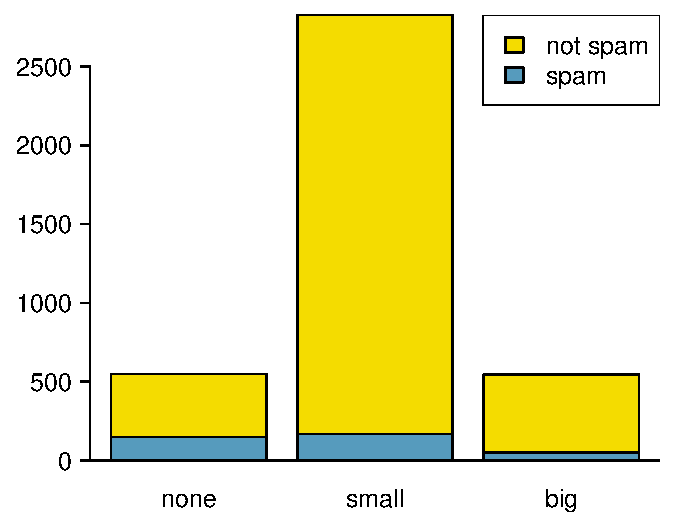
\includegraphics[width=0.46\textwidth]{01/figures/emailSpamNumberSegBar/emailSpamNumberSegBar}
\label{emailSpamNumberSegBar} %typeDriveTrainSegBarPlotOrig}
}
\subfigure[]{
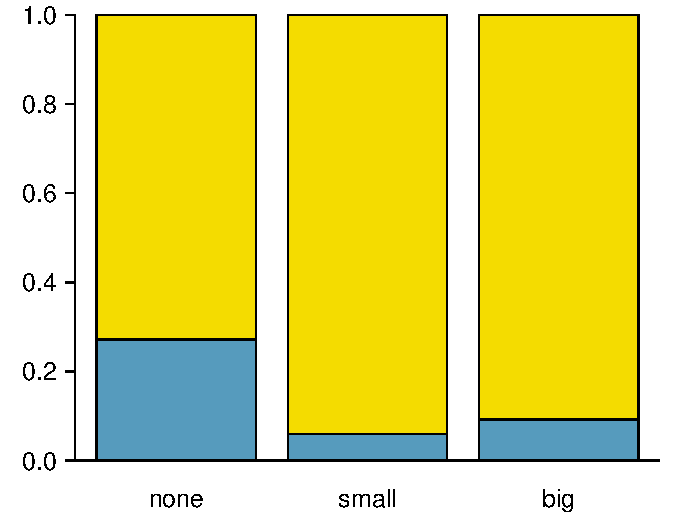
\includegraphics[width=0.46\textwidth]{01/figures/emailSpamNumberSegBar/emailSpamNumberSegBarSta}
\label{emailSpamNumberSegBarSta} %typeDriveTrainSegBarPlotSta}
}
\caption{\subref{emailSpamNumberSegBar} Segmented bar plot for numbers found in emails, where the counts have been further broken down by \var{spam}. \subref{emailSpamNumberSegBarSta} Standardized version of Figure~\subref{emailSpamNumberSegBar}.}
\label{emailSpamNumberSegBarPlot} % typeDriveTrainSegBarPlot}
\end{figure}

The choice to describe each level of \var{spam} within the levels of the \var{number} variable was for the same reason we would prefer column proportions of Table~\ref{emailSpamNumberTableTotals}: it is more interesting to see how many emails in each level of \var{number} are spam. Just like considering row and column proportions, it is helpful to think carefully about the best way to construct a segmented bar plot before choosing a final form.

\begin{example}{Examine both of the segmented bar plots. Which is more useful?}
Figure~\ref{emailSpamNumberSegBar} contains more information, but Figure~\ref{emailSpamNumberSegBarSta} presents the information more clearly. This second plots helps make it clear that emails with no number or with a very big number have a relatively high fraction of email. Since the fraction of spam changes across the groups, we can conclude the variables are dependent (something we also were able to discern using the row or column proportions in the Tables~\ref{rowPropSpamNumber} and~\ref{colPropSpamNumber}). Because spam is such a small fraction of email in any of the groups, this is more difficult to see in Figure~\ref{emailSpamNumberSegBar}.

In some other cases, a segmented bar plot that is not standardized will be more useful in communicating important information. If you will use a segmented bar plot, we recommend you look at both type before settling on a final form.
\end{example}

\begin{figure}[p]
\centering
\subfigure[]{
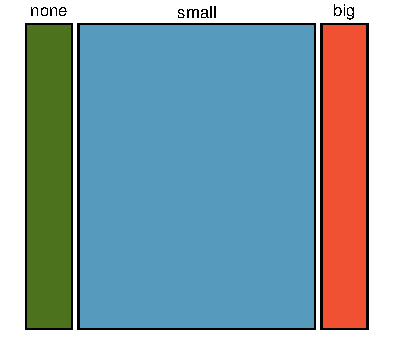
\includegraphics[width=0.4246\textwidth]{01/figures/emailSpamNumberMosaicPlot/emailNumberMosaic}
\label{emailNumberMosaic}
}
\subfigure[]{
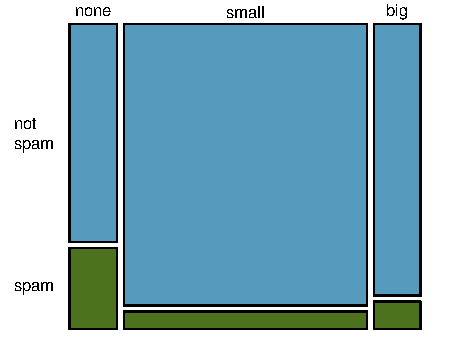
\includegraphics[width=0.4954\textwidth]{01/figures/emailSpamNumberMosaicPlot/emailSpamNumberMosaic}
\label{emailSpamNumberMosaic}
}
\caption{The one-variable mosaic plot for \var{number} and the two-variable mosaic plot for both \var{number} and \var{spam}.}
\label{emailSpamNumberMosaicPlot}
\end{figure}

\begin{figure}
   \centering
   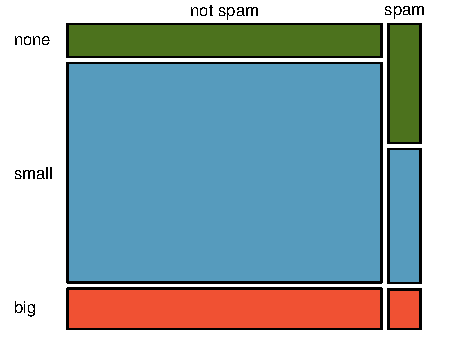
\includegraphics[width=0.65\textwidth]{01/figures/emailSpamNumberMosaicPlot/emailSpamNumberMosaicRev}
   \caption{Mosaic plot where emails are broken up by the \var{number} variable after they've been divided into \resp{spam} and \resp{not spam}.}
   \label{emailSpamNumberMosaicRev}
\end{figure}

A \term{mosaic plot} is a graphical display of contingency table information that is similar to a bar plot for one variable or a segmented bar plot when using two variables. Figure~\ref{emailNumberMosaic} shows a mosaic plot for the \var{number} variable from Table~\ref{emailSpamNumberTableTotals}. Each column represents a level of \var{number}, and the column widths correspond to the proportion of emails of each number type. For instance, there are fewer emails with no numbers than emails with only small numbers, so the no number email column is slimmer. In general, mosaic plots use box \emph{areas} to represent the number of observations that box represents.

This one-variable mosaic plot is further broken into pieces in Figure~\ref{emailSpamNumberMosaic} using the \var{spam} variable. Each column is split proportionally according to the fraction of emails that were spam in each number category. For example, the second column, representing emails with only small numbers, was broken into emails that were spam (lower) and not spam (upper). 
As another example, the bottom of the third column represents spam emails that had big numbers (perhaps from a someone needing to wire money from Nigeria), and the upper part of the third column represents regular emails that had big numbers. We can again use this plot to see that the \var{spam} and \var{number} variables are associated since each column is broken apart in different vertical locations, which was the same technique used for the standardized version of the segmented bar plot.

In a similar way, a mosaic plot representing row proportions of Table~\ref{emailSpamNumberTableTotals} could be constructed, as shown in Figure~\ref{emailSpamNumberMosaicRev}. However, because it is more insightful for this application to consider the fraction of spam in each category of the \var{number} variable, we prefer Figure~\ref{emailSpamNumberMosaic}.

\begin{exercise}
Describe how the mosaic plot shown in Figure~\ref{emailSpamNumberMosaicRev} was constructed. Answer in the footnote\footnote{First, emails were split into those that were spam and those that were not spam, represented by the two columns. Then the \var{number} variable splits each of these columns into three levels \resp{none}, \resp{small}, and \resp{big}.}.
\end{exercise}

\subsection{The only pie chart you will see in this book}

While pie charts are well known, they are not typically as useful as other charts in a data analysis. A \term{pie chart} is shown in Figure~\vref{emailNumberPieChart} alongside a bar plot. It is generally more difficult to compare group sizes in a pie chart than in a bar plot, especially when categories have nearly identical counts or proportions. %In this particular case, we actually may be better off skipping a chart altogether and providing a table since only 3 values are needed and a table can provide much greater precision.
\begin{figure}%[bth]
   \centering
   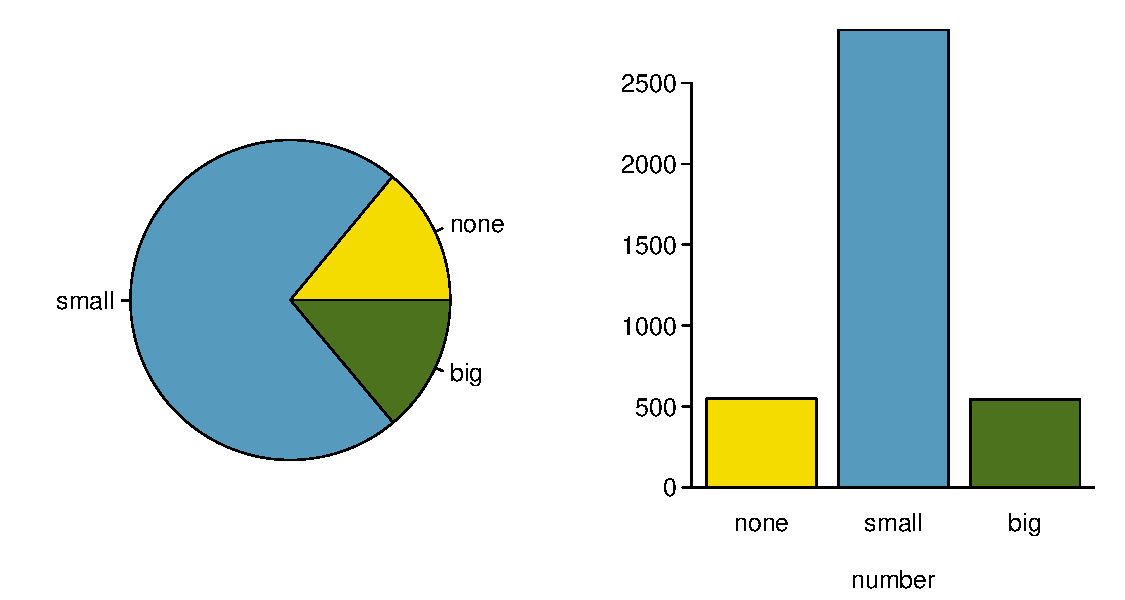
\includegraphics[width=0.88\textwidth]{01/figures/emailNumberPieChart/emailNumberPieChart}
   \caption{A pie chart and bar plot of \var{number} for the \data{email} data set.}
   \label{emailNumberPieChart}%carsTypePieChart}
\end{figure}

\index{data!email|)}

\subsection{Comparing numerical data across groups}
\label{comparingAcrossGroups}

\index{data!county|(}

Some of the more interesting investigations can be considered by examining numerical data across groups. The methods required here aren't really new. All that is required is to make a numerical plot for each group. Here two convenient methods are introduced: side-by-side box plots and hollow histograms.

We will take a look again at the \data{county} data set and examine whether there is evidence that counties that lose population from 2000 to 2010 versus counties that have a steady or increasing population over those ten years have higher or lower homeownership rates. While we might like to make a causal connection here, remember that these are observational data and so such an interpretation would be unjustified.

%So perhaps people are leaving the county because of higher poverty rates, or perhaps higher poverty rates are caused by a county being partially deserted.

There were 2,041 counties that increased their population and 1,099 with no gain (all but one were a loss). A~random sample of 100 counties from the first group and 50 from the second group are shown in Table~\ref{countyIncomeSplitByPopGainTable} to give a better sense of some of the raw data.
\begin{table}
\centering\small
\begin{tabular}{ ccc ccc c ccc }
\multicolumn{6}{c}{\bf population gain} && \multicolumn{3}{c}{\bf no gain} \\ 
  \cline{1-6} \cline{8-10}
41.2 & 33.1 & 30.4 & 37.3 & 79.1 & 34.5 &\hspace{5mm}\ & 40.3 & 33.5 & 34.8 \\
22.9 & 39.9 & 31.4 & 45.1 & 50.6 & 59.4 && 29.5 & 31.8 & 41.3 \\
47.9 & 36.4 & 42.2 & 43.2 & 31.8 & 36.9 && 28 & 39.1 & 42.8 \\
50.1 & 27.3 & 37.5 & 53.5 & 26.1 & 57.2 && 38.1 & 39.5 & 22.3 \\
57.4 & 42.6 & 40.6 & 48.8 & 28.1 & 29.4 && 43.3 & 37.5 & 47.1 \\
43.8 & 26 & 33.8 & 35.7 & 38.5 & 42.3 && 43.7 & 36.7 & 36 \\
41.3 & 40.5 & 68.3 & 31 & 46.7 & 30.5 && 35.8 & 38.7 & 39.8 \\
68.3 & 48.3 & 38.7 & 62 & 37.6 & 32.2 && 46 & 42.3 & 48.2 \\
42.6 & 53.6 & 50.7 & 35.1 & 30.6 & 56.8 && 38.6 & 31.9 & 31.1 \\
66.4 & 41.4 & 34.3 & 38.9 & 37.3 & 41.7 && 37.6 & 29.3 & 30.1 \\
51.9 & 83.3 & 46.3 & 48.4 & 40.8 & 42.6 && 57.5 & 32.6 & 31.1 \\
44.5 & 34 & 48.7 & 45.2 & 34.7 & 32.2 && 46.2 & 26.5 & 40.1 \\
39.4 & 38.6 & 40 & 57.3 & 45.2 & 33.1 && 38.4 & 46.7 & 25.9 \\
43.8 & 71.7 & 45.1 & 32.2 & 63.3 & 54.7 && 36.4 & 41.5 & 45.7 \\
71.3 & 36.3 & 36.4 & 41 & 37 & 66.7 && 39.7 & 37 & 37.7 \\
50.2 & 45.8 & 45.7 & 60.2 & 53.1 &  && 21.4 & 29.3 & 50.1 \\
35.8 & 40.4 & 51.5 & 66.4 & 36.1 &  && 43.6 & 39.8 &  \\
\cline{1-6} \cline{8-10}
\end{tabular}
\caption{In this table, homeownership rates of a random sample of 100 counties that held steady or gained population over 2000-2010 are shown on the left, and rates for a sample of 50 counties that had a lower population are shown on the right.}
\label{countyIncomeSplitByPopGainTable}
\end{table}

The \term{side-by-side box plot} \index{box plot!side-by-side box plot} is a traditional tool for comparing across groups. An example is shown in the left panel of Figure~\ref{countyIncomeSplitByPopGain}, where there are two box plots -- one for each group -- placed into one plotting window and drawn on the same scale.
\begin{figure}
   \centering
   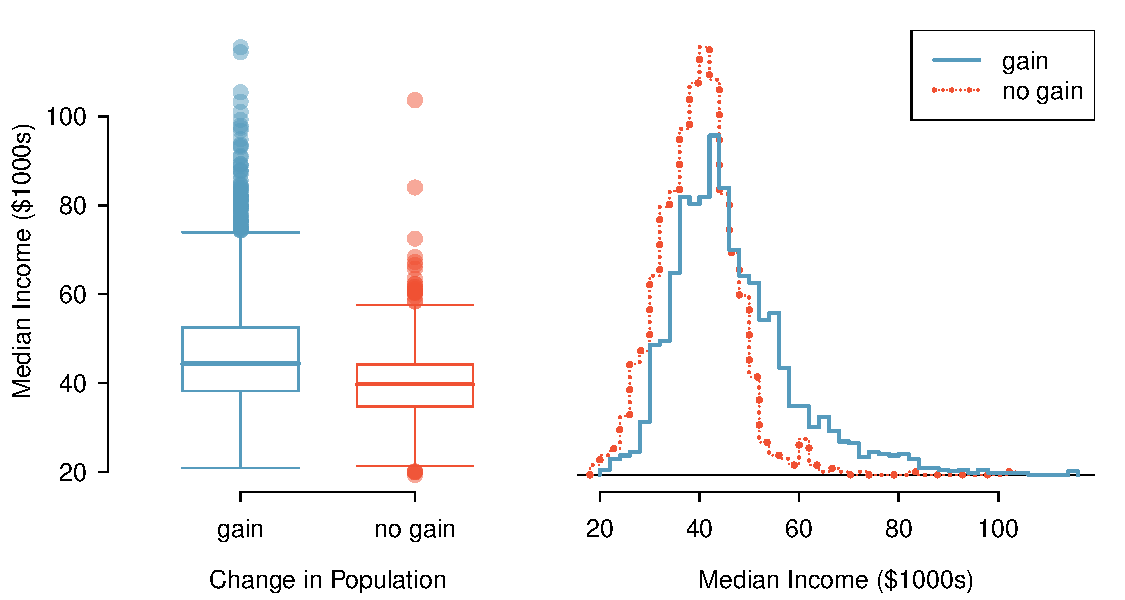
\includegraphics[width=0.85\textwidth]{01/figures/countyIncomeSplitByPopGain/countyIncomeSplitByPopGain}
   \caption{Side-by-side box plot (left panel) and hollow histograms (right panel) for \var{home\_ownership} where the counties are split by whether there was a population gain or loss over the 2000 to 2010. The home ownership rate was taken in 2010.}
   \label{countyIncomeSplitByPopGain}
\end{figure}

\termsub{Hollow histograms}{hollow histograms} are another useful plotting method for numerical data being compared across groups. These are just the outlines of histograms of each group put on the same plot, as shown in the right panel of Figure~\ref{countyIncomeSplitByPopGain}.

\begin{exercise} \label{comparingPriceByTypeExercise}
Use each plot in Figure~\ref{countyIncomeSplitByPopGain} to compare the median incomes for counties across the two groups. What do you notice about the approximate center of each group? What do you notice about the variability between groups? Is the shape relatively consistent between groups? How many \emph{prominent} modes are there for each group? Answers in the footnote\footnote{Answers may vary a little. The counties with population gains tend to have higher income (median of about \$45,000) versus counties without a gain (median of about \$40,000). The variability is also slightly larger for the \emph{population gain}, group which is evident in the IQR, which is about 50\% bigger in the \emph{gain} group. Both distributions show modest right skew and are unimodal. There is a seconary small bump at about \$60,000 for the \emph{no gain} group, visible in the hollow histogram plot, that seems out of place. (Looking into the data set, we would find that 8 of these 15 counties are in Alaska and Texas.) The box plots indicate there are many apparent outliers in each group on the high ends, though we should anticipate that many observations will fall beyond the whiskers when using such a large data set.}.
\end{exercise}

\begin{exercise}
What components of each plot in Figure~\ref{countyIncomeSplitByPopGain} do you find most useful? Answer in the footnote\footnote{Answers will vary. The side-by-side box plots are especially useful for comparing centers and spreads, while the hollow histograms are more useful for seeing distribution shape, skew, and groups of anomalies.}.
\end{exercise}

\index{data!county|)}



%%%%%
%\section{Exploratory graphics}
%\label{exploratoryGraphicsSection}
%
%Many interesting analyses draw on multiple sources or creative representations of graphics. This sections three graphical explorations of the 2008-9 financial crisis, the relationship among and 2011-2012 GOP presidential nomination race, and three variables of the \data{states} data set: \var{smoking}, \var{murder}, and \var{coalEnergy} (the percent of a state's energy that comes from coal).
%
%So far we have focused largely on one source of data at a time. Many of the most interesting analyses and insights are generated by merging data across sources.
%
%\subsection{2008-9 financial crisis}
%
%In this section, we combine Wikipedia data with financial data to consider the impact financial markets had on the public's interest in understanding what is a \emph{financial crisis}. Wikipedia's traffic is publicly available on \href{http://stats.grok.se/}{stats.grok.se}, and stock information can be downloaded from a website like \href{http://www.google.com/finance}{Google Finance} or \href{http://finance.yahoo.com/}{Yahoo! Finance}. We will take a look at why one might be interested in merging these data.
%
%Figure~\ref{wikipediaStocks} shows visit's to  \href{http://en.wikipedia.org/wiki/Financial_crisis}{Wikipedia's Financial Crisis page} and the Dow Jones Industrial Average (DJI) from late 2007 until early 2012. The DJI is a stock index and is a good indicator of a large number of stocks. That is, if it goes down, that means many stocks also went down, and so on.
%\begin{figure}
%   \centering
%   \includegraphics[width=\textwidth]{01/figures/wikipediaStocks/wikipediaStocks}
%   \caption{The vertical lines show the number of daily views of Wikipedia's Financial Crisis page from late 2007 to early 2012, where the scale . Any regions with missing spikes indicate dates where data is missing. The continuous line that dips and rises represents the daily closing price of the Dow Jones Industrial Average, which represents.}
%   \label{wikipediaStocks}
%\end{figure}
%% Peak	2007-10-09	14,164.53
%% 		2008-09-01	11,543.55 (round to 11,500 since this was a weekend)
%%		2008-10-01
%
%Let's take the data separately before we analyze their joint information. In the DJI, a general decline in stocks is evident until a bottoming out in the first quarter of 2009. From there forward, there is a general increase in the index, albeit the increase is regularly interrupted by drops in price.
%
%The page view data tells another interesting account of the financial crisis. There were few visitors to the financial crisis page until late 2008 when views soared. There was a peak in visitors before 2009, which declined to an elevated but much more stable number of views in mid-2009.
%
%If the combined data is actually shocking. The financial crisis page views occurred immediately before the steepest sell-offs. The first day with more than 1000 page views was September 1st when the DJI was off by 19\% from its October 2007 peak (14,165). By October 15th, 2008, the DJI would drop a further 21\%, at which point page views were soaring to over 4000 each day, up from the August average of 203 page views each day. By the time the DJI index bottomed out, it lost over 53\% of its
%
%The story told by these data is intriguing. Based on this example, it might be tempting to predict stock movements or other outcomes based on page view data. We want to temper this sentiment a little by noting that other page views may not always be so clear. For instance, a company's Wikipedia page may have a surge in views, which might indicate success, dramatic failure, or nothing of meaningful whatsoever. As we learned in Section~\ref{}, trying to identify causal relationships from observational data is at best, very difficult, and at worst, impossible.
%
%
%%\subsection{GOP presidential nomination race}
%
%\subsection{Debt ceiling deadline}
%
%Summer 2011 saw one of the most heated and controversial political battles that roiled global financial markets and contributed to the first downgrade of United States debt. We can take a glimpse inside of the political back-and-forth by examining the Twitter profiles of three of the most prominent political players in the debate: President Barack Obama, Speaker John Boehner, and Senate Minority Leader Mitch McConnell. Figure~\ref{} shows their weekly number of Twitter posts.
%
%
%%\subsection{Mapping state data}



%%%%%%%%%%%%%%%%%%%%%%%%%%%%%%%%%%%%%%%%%%%%

\section{Case study: gender discrimination (special topic)}
\label{caseStudyGenderDiscrimination}

%%%%%%%%%%%%%%%%%%%%%%%%%%%%%%%%%%%%%%%%%%%%

\begin{example}{Suppose your professor splits the students in class into two groups: students on the left and students on the right. If $\hat{p}_{_L}$ and $\hat{p}_{_R}$ represent the proportion of students who own an Apple product on the left and right, respectively, would you be surprised if $\hat{p}_{_L}$ did not {exactly} equal $\hat{p}_{_R}$?}\label{classRightLeftSideApple}
While the proportions would probably be close to each other, it would be unusual for them to be exactly the same. We would probably observe a small difference due to {chance}.
\end{example}

\begin{exercise}
If we don't think the side of the room a person sits on in class is related to whether the person owns an Apple product, what assumption are we making about the relationship between these two variables?
Answer in the footnote\footnote{We would be assuming that these two variables are independent.}.
\end{exercise}

%%%%%%%%%%%%%%%%%%%%%%

\subsection{Variability within data}
\label{variabilityWithinData}

%%%%%%%%%%%%%%%%%%%%%%

In this first section, we consider a study investigating the influence of sex role stereotypes on the personnel decisions of bank supervisors\footnote{B. Rosen and T. Jerdee, ``Influence of sex role stereotypes on personnel decisions.," Journal of Applied Psychology, 59(1), 1974.}. \citep{Rosen:1974} One of the research questions evaluated in this study that we hope to answer is ``Are females unfairly discriminated against in promotion decisions made by male managers?"

The participants in this study are 48 male bank supervisors attending a management institute at the University of North Carolina during the summer of 1972. They were asked to assume the role of the personnel director of a bank and were given the same personnel file to judge whether the person should be promoted to a branch manager position. The files given to the participants were identical, except that half of them indicated that the person was male and the other half female. These files were randomly assigned to the subjects.

\begin{exercise}
Is this an observational study or an experiment? What implications does the type of the study have on what can be inferred from the results?
Answer in the footnote\footnote{The study is an experiment, subjects are randomly assigned whether or not they get a male or female file. Since this is an experiment, the results can be used to suggest a causal relationship between gender and promotion decision.}.
\end{exercise}

For each file we record the \var{gender} and the \var{promotion decision}. Using the results of the study summarized in Table~\ref{discriminationResults} we would like to evaluate if females are unfairly discriminated against in promotion decisions. In this study, a smaller proportion of females are promoted than males (0.875 versus 0.583), however, it is unclear whether that difference provides \emph{convincing evidence} that females are unfairly discriminated against.
\begin{table}[ht]
\centering
\begin{tabular}{l l cc rr}
& & \multicolumn{2}{c}{\var{promotion decision}} \\
  \cline{3-4}
		&			& 	\resp{promoted} 	& \resp{not promoted} & Total & \hspace{3mm}  \\ 
  \cline{2-5}
		&	\resp{male} 			& 21    		& 3   & 24  	 \\ 
  \raisebox{1.5ex}[0pt]{\var{gender}}		&	\resp{female} 	& 14    		& 10     & 24	 \\ 
  \cline{2-5}
  		&	Total		& 35	& 13	&  48 \\
  \cline{2-5}
\end{tabular}
\vspace{-2mm}
\caption{Summary results for the gender discrimination study.}
\label{discriminationResults}
\end{table}

\begin{example}{Statisticians are sometimes called upon to evaluate the strength of evidence. When looking at the rates of promotion for males and females in this study, what comes to mind as we try to determine whether the data show convincing evidence of a real difference?} \label{discriminationResultsWhatIsConvincingEvidence}
The observed promotion rates (87.5\% for males versus 58.3\% for females) suggest that there might be unfair discrimination against women in promotion decisions. However, we cannot be sure, simply by comparing the observed proportions, if the difference is real or due to chance. Generally there is a little bit of fluctuation in sample data, and we wouldn't expect the sample proportions to be \emph{exactly} equal even if the truth was that they were equal for males and females. As we look at the data, we want to ask, is the difference between the promotion rates so large that it probably isn't due to chance?
\end{example}

Example~\exam{discriminationResultsWhatIsConvincingEvidence} is a reminder that the observed outcomes in the sample may not perfectly reflect the true relationships between variables in the underlying population. Table~\ref{discriminationResults} shows there were 7 fewer promotions in the female group than in the male group, a difference in promotion rates of 29.2\% $\left( \frac{21}{24} - \frac{14}{24} = 0.292 \right)$. This difference between is not small, but the sample size for the study is not large, and hence it's unclear if this observed difference is indicative of a real relationship between gender and promotion decisions, or simply due to chance. We label these two competing claims, $H_0$ and $H_A$:
\begin{itemize}
\setlength{\itemsep}{0mm}
\item[$H_0$:] \textbf{Independence model.} The variables \var{gender} and \var{decision} are independent. They have no relationship, and the observed difference between the proportion of males and females who got promoted, 29.2\%, was due to chance.
\item[$H_A$:] \textbf{Alternative model.} The variables \var{gender} and \var{decision} are \emph{not} independent. The difference in promotion rates of 29.2\% was not due to chance and equally qualified females are less likely to be promoted than males.
\end{itemize}

What it would mean if the independence model, which says that the variables \var{gender} and \var{decision} are unrelated, is true? Each file was either going to be deemed eligible for promotion, and the gender indicated on the file had no effect on the outcome. The researchers were just randomly splitting these files into two groups, very much like we split the class in half in Example~\exam{classRightLeftSideApple}. If this was the case, the difference of 29.2\% the researchers observed would be simply due to chance.

Consider the alternative: gender indicated on the file affects the promotion decision. If this is true, we would expect to see some difference in the promotion rates of males and females, with a lower percentage of promotion in the among the files that were marked as female.

We choose between these two competing claims by assessing if the data conflict so much with $H_0$ that the independence model cannot be deemed reasonable that we should reject it in favor the alternative model, $H_A$. In other words, we start by assuming that there is no relationship between the two variables, $H_0$ is true, and keep that position unless the evidence from the study in favor of $H_A$ is extremely convincing.

%%%%%%%%%%%%%%%%%%%%%%

\subsection{Simulating the study}

%%%%%%%%%%%%%%%%%%%%%%

Suppose $H_0$ is true. Under this model, the 29.2\% difference would have been due to chance, and the gender indicated on the files would not have impacted promotion decisions. We can assess how likely it is to get such a difference between the promotion rates of males and females just by random chance by simulating differences using a \term{randomization technique}.

We are going to recreate (simulate) the study under the scenario that the promotion decision is not affected by the gender indicated on the files. We can run this \term{simulation} by taking 35 index cards labeled \var{promoted} and 13 index cards labeled \var{not promoted}\footnote{You can also do this using playing cards. From a full deck of 52 cards take out 3 aces and one number card. You'll be left with 13 face cards representing not promoted files, and 35 number cards representing promoted files. If you have access to a deck of cards, give it a try.}. Then, we shuffle the cards and split them into two groups of equal sizes: a group of 24 cards indicating a simulated (fake) male group and the other 24 indicating a simulated female group. Then, since we know this simulated group assignment has nothing to do with the actual promotion decisions -- the simulated group assignment and the promotion decision are independent -- any observed difference in promotion rates between the simulated groups must be due to chance.

We can also do the simulation using a computer program and randomly assigning labels \var{maleSim} and \var{femaleSim} to the personnel files. Results of such a simulation are presented in Table~\ref{discriminationRand1}.
\begin{table}[ht]
\centering
\begin{tabular}{l l cc rr}
& & \multicolumn{2}{c}{\var{decision}} \\
  \cline{3-4}
		&			& 	\resp{promoted} 	& \resp{not promoted} & Total & \hspace{3mm}  \\ 
  \cline{2-5}
		&	\resp{maleSim} 					& 18    		& 6    & 24 	 \\ 
  \raisebox{1.5ex}[0pt]{\var{genderSim}}		&	\resp{femaleSim} 	& 17    		& 7 & 24    	 \\ 
  \cline{2-5}
  & Total	& 35 & 13 & 48
\end{tabular}
\caption{Simulation results, where any difference in promotion rates between \resp{maleSim} and \resp{femaleSim} is purely due to chance.}
\label{discriminationRand1}
\end{table}

\begin{exercise} \label{sampleDifferenceInMaleAndFemaleDiscrimination}
What is the difference in promotion rates between the two simulated groups in Table~\ref{discriminationRand1}? How does this compare to the observed 29.2\% in the actual groups? Answer in the footnote\footnote{$18/24 - 17/24=0.042$ or about 4.2\%. This difference due to chance is much smaller.}.
\end{exercise}

%%%%%%%%%%%%%%%%%%%%%%

\subsection{Checking for independence}

%%%%%%%%%%%%%%%%%%%%%%

We computed one possible difference under the independence model in Exercise~\exer{sampleDifferenceInMaleAndFemaleDiscrimination}, which represents one difference due to chance. We could repeat the simulation to get another difference from chance: -0.125. And another: -0.042. And another: 0.208. And so on until we repeat the simulation enough times that we have a good idea of what represents the \emph{distribution of differences from chance alone}. Figure~\ref{discRandDotPlot} shows a plot of the differences found from 100 simulations where each dot represents a simulated difference between the proportions of male and female files that were deem end eligible for promotion.
\setlength{\captionwidth}{\mycaptionwidth+3mm}
 \begin{figure}[ht]
    \centering
    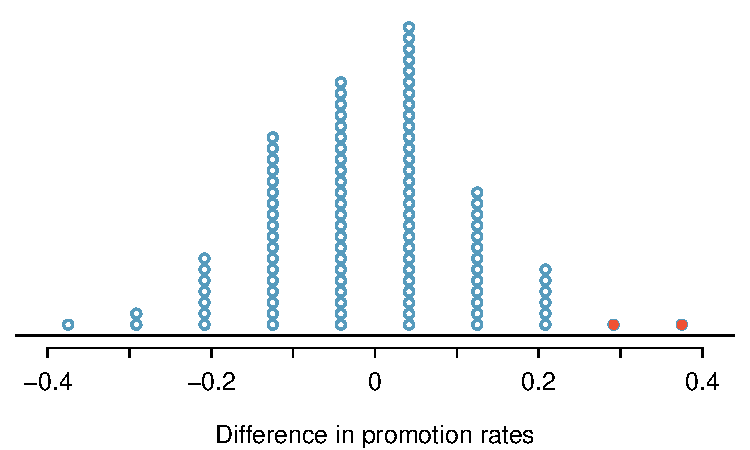
\includegraphics[width=0.7\textwidth]{01/figures/discRandDotPlot/discRandDotPlot}
    \caption{A dot plot of differences from 100 simulations produced under the independence model, $H_0$, where \var{genderSim} and \var{decision} are independent. Two of the one-hundred simulations had a difference of at least 29.2\%.}
    \label{discRandDotPlot}
 \end{figure}
\setlength{\captionwidth}{\mycaptionwidth}

Note that the distribution of these simulated differences are centered around 0. We simulated these differences assuming that the null hypothesis, the independence model, was true. If so, we wouldn't expect there to be any difference between the proportions of males and females who get promoted, hence yielding a difference of 0 between the promotion rates. However, each time we simulate the study, we don't expect to get a difference of exactly 0. Sometimes, just by chance, the difference is higher than 0, indicating more promoted files end up in the simulated male group, and sometimes it's lower, indicating the opposite. 

\begin{example}{How often would you observe a difference of at least 29.2\% (0.292) according to Figure~\ref{discRandDotPlot}? Often, sometimes, rarely, or never?}
It appears that a difference of at least 29.2\% due to chance alone would only happen about 2\% of the time according to Figure~\ref{discRandDotPlot}. Such a low probability indicates a rare event.
\end{example}

The difference of 29.2\% being a rare event suggests two possible interpretations of the results of the study:
\begin{itemize}
\setlength{\itemsep}{0mm}
\item[$H_0$] \textbf{Independence model.} Gender has no effect on promotion decision, and we observed a difference that would only happen rarely.
\item[$H_A$] \textbf{Alternative model.} Gender has an effect on promotion decision, and what we observed was actually due to equally qualified women being unfairly discriminated against in promotion decisions, which explains the large difference of 29.2\%.
\end{itemize}
We should be skeptical that what was observed is considered a rare event, hence reject the null hypothesis in favor of the alternative. In this situation we would conclude that the data provide convincing evidence of gender discrimination against women in promotion decisions.

One field of statistics, statistical inference, is built on evaluating whether such differences are due to chance. In statistical inference, statisticians evaluate which model is most reasonable given the data. Errors do occur -- we might choose the wrong model. While we do not always choose correctly, statistical inference gives us tools to control and evaluate how often these errors occur. In Chapter~\ref{foundationsForInference}, we give a formal introduction to the problem of model selection. However, we spend the next two chapters building a foundation of probability and theory necessary to make that discussion rigorous.
